\documentclass[journal]{IEEEtran}
%\documentclass[onecolumn]{IEEEtran}
\usepackage{multirow}
\usepackage{algorithm}
\usepackage{color}
\usepackage{url}
\usepackage{times}
\usepackage{graphicx}
\usepackage{float}
\usepackage{epstopdf}
\usepackage{amsmath}
\usepackage{amssymb}
\usepackage{algorithmicx}
\usepackage{algpseudocode}
\usepackage{bm}
\usepackage{subfigure}
%\usepackage{subfig}
% Load basic packages
\usepackage{balance}  % to better equalize the last page
\usepackage{graphics} % for EPS, load graphicx instead
\usepackage{bm}
\usepackage{tabularx}
\usepackage{booktabs}
\usepackage{threeparttable}
\usepackage{indentfirst}
\usepackage{array}
\usepackage{color}
%\usepackage[justification=centering]{caption}
\usepackage{booktabs}

\hyphenation{op-tical net-works semi-conduc-tor}

\newcommand{\name}{RFL}
\newcommand{\namekey}{RSKey}

\begin{document}
%
% paper title
% can use linebreaks \\ within to get better formatting as desired
\title{\name{}: Robust Fault Localization on Unreliable Communication Channels}

\iffalse
\author{
\IEEEauthorblockN{Bo Wu\IEEEauthorrefmark{1},  Ke Xu\IEEEauthorrefmark{1}, Qi Li\IEEEauthorrefmark{1}, Fan Yang\IEEEauthorrefmark{1}}

\IEEEauthorblockA{\IEEEauthorrefmark{1}Department of Computer Science and Technology, Tsinghua University, Beijing, China \\Emails: {wub14@mails.tsinghua.edu.cn, xuke@tsinghua.edu.cn, qi.li@sz.tsinghua.edu.cn, y-f14@tsinghua.org.cn}}
%\IEEEauthorblockA{\IEEEauthorrefmark{2}Tsinghua National Laboratory for Information Science and Technology, Tsinghua University, Beijing, China}
}
\fi

\author{\IEEEauthorblockN{}
\IEEEauthorblockA{Bo Wu, \emph{Member}, \emph{IEEE}, Ke Xu, \emph{Senior Member}, \emph{IEEE}, Qi Li, \emph{Senior Member}, \emph{IEEE},\\ Fan Yang, and Kui Ren, \emph{Fellow}, \emph{IEEE}}

\thanks{Bo Wu, Ke Xu, Qi Li and Fan Yang are with the Department of Computer Science and Technology, Tsinghua University, Beijing, China. They are also with the Tsinghua National Laboratory for Information Science and Technology, Beijing 100084, China. (Email: wub14@mails.tsinghua.edu.cn, xuke@tsinghua.edu.cn, qi.li@sz.tsinghua.edu.cn, y-f14@tsinghua.org.cn).}
\thanks{Kui Ren is with the Institute of Cyber Security Research, Zhejiang University, China. (Email: kuiren@zju.edu.cn).}
}

% make the title area
\maketitle


\begin{abstract}
The current Internet is vulnerable to various attacks, e.g., source spoofing and flow hijacking attacks, which are incurred by misconfigurations or attacks. Either users or network operators are unable to easily localize these faults. Existing fault localization mechanisms can detect such attacks under an assumption that localization is performed upon reliable communication channels. Unfortunately, the assumption does not always  hold. The forwarding paths of localization are not always reliable. Packets are always dropped for some reasons. In particular, adversaries can interfere with the fault localization by maliciously dropping packets.  In this paper, we relax the assumption and propose a robust data-plane fault localization protocol, i.e., \name{},  
%\textcolor{red}{source and path verification protocol} 
that can localize faults and achieve source authenticity and path compliance even if communication channels in the network are not reliable. \name{} samples and signs packets in each network entity so that the packet source can efficiently localize faults of packet forwarding by verifying the sampled packets. %In particular, 
By leveraging packet acknowledgment, packet sampling based fault localization is not impacted by packet loss in the communication channels. %the reliability of the communication channels. 
\textcolor{red}{In particular, \name leverages a symmetric key distribution scheme to implement robust key distribution among different entities, which ensures that packet sources can always correctly fresh their keys to perform correct localization.} 
%For enhancing reliable packet delivery, we present a robust fault localization scheme, named \name{}, to localize the misbehaved entity.} %\name{} uses symmetric keys to build secure detection channels and 
%\textcolor{red}{Based on acknowledgements from entities, \name{} and \namekey{} can enable the source to localize the fault during symmetric key distribution and packet delivery, which are} %enables packets sampling for localization on the channels such that it can detect and localize faults. In particular, the localization performed is 
%not impacted by the reliability of the communication channels, e.g., the packets used to localize faults are dropped. 
\textcolor{red}{Our security and theoretical analysis proves the robustness of RFL protocol.} We implement the  \name{} prototype on the Click routers. The experiment results with the prototype demonstrate that \name{} achieves more than 99.5\% localization accuracy, while incurring only 10\% throughput degradation. 
%The current network is vulnerable to the source spoofing and flow hijacking attacks caused by compromised/misconfigured router. Both users and network operators are all powerless to localize the fault when any error occurs. Existing fault localization mechanisms cannot achieve a practical tradeoff between security and robustness, and require a unacceptably reliable transmission channel. In this paper, we propose a robust and lightweight data-plane fault localization protocol called RLFL for source authenticity and path compliance. RLFL provides anti-attack symmetric key distribution and fault localization in unreliable transmission channel, and lightweight router storage overhead of only 3.23 MB. We implemented prototype of RLFL on Linux/Click router, which achieves over 90\% throughput and approximate 85\% goodput of baseline. Our simulation results shows a higher localization accuracy of over 99.5\% while retaining a high level of security.

%\boldmath
%The current Internet is vulnerable to various types of the inconsistency between data plane and control plane, due to either malicious attacks, such as source spoofing and flow hijacking, or network misconfiguration, such as operator's incorrect manipulation. Unfortunately, some simple methods like ping, traceroute, etc. could not satisfy the requirement to monitor and localize this inconsistency as the possible existence of malicious intermediate router(s). Consequently, there is no reliable assurance provided for the current network to monitor this inconsistency, allowing counterfeited packet origins, eavesdropping private information and increased transmission overhead. Thus, detecting the data-plane source authenticity and path compliance is high desired to identify, locate the misbehaver 
\end{abstract}
\begin{IEEEkeywords}
Symmetric Key Distribution, Source and Path Verification, Fault Localization
\end{IEEEkeywords}

\section{Introduction}
Reliable data delivery is highly desirable for Internet users, in particular, for security-critical services enabled in ISPs, enterprises, and datacenter networks \cite{zeng2012automatic}, which requires correct packet delivery along the desired forwarding paths and with the authentic origin. 
However, the current design of Internet always suffers from packet source spoofing and traffic hijacking attacks. % due to the existence of misconfiguration or attacks. %These network vulnerabilities are commonly used by attackers for carrying out malicious activities, such as Man in the middle (MiTM) \cite{desmedt2011man}, DoS/DDoS attacks (e.g., refection \cite{reflectionattack} and DNS amplification \cite{dnsamplificationattack}) and traffic redirection. 
It is difficult to identify such attacks in real time. 
Existing troubleshooting tools, e.g., ping and traceroute, cannot effectively identify and localize faults.  Various attacks can be launched to generate packets with fake packet origins and hijack forwarding path~\cite{kim2014lightweight}. %, and eavesdrop private information. 
Thus, it is necessary to enable data-plane fault localization to ensure correct packet forwarding on the Internet.
%for source and path verification is an essential remediation for securing data delivery.\\
%In this case, many attacks can be launched to counterfeit packet origins, change forwaarding path, eavesdrop private information, and increase transmission overhead.\\
%The current Internet is vulnerable to various types of the inconsistency between data plane and control plane, due to either malicious attacks, such as source spoofing and flow hijacking, or network misconfiguration, such as operator's incorrect manipulation. Unfortunately, some simple methods like ping, traceroute, etc. can not satisfy the requirement to detect and localize this inconsistency as the malicious intermediate router(s) can disturb (drop, modify) the detection packets. Consequently, there is no reliable assurance provided for the current network to detect this inconsistency, allowing counterfeited packet origins, eavesdropping private information and increased transmission overhead. Thus, detecting the data-plane source authenticity and path compliance is high desired to identify, localize the misbehaver \cite{zeng2012automatic}. By repairing or avoiding the misbehaved router from the forwarding path, many attacks caused by this inconsistency can be mitigated, bring more secure end-to-end communication.
%\vspace{-0.03cm}

%\textcolor{red}{In particular, under unreliable communication channels, which allows network entities on it to interfere with fault localization by dropping, modifying and redirecting packets.} 

%\indent
In order to address this issue, end-to-end source authentication \cite{liu2008passport} \cite{perrig2001efficient} and path validation \cite{parno2008snapp} \cite{zhao2005aggregated} \cite{kent2000secure} have been extensively studied. %to mitigate the source spoofing and path
% inconsistency attacks.
They verify packet origins and forwarding paths by embedding cryptographic tags (or markings) to localize faults in packet forwarding. 
However, they assume that the packets used to verify markings can be correctly delivered over reliable communication channels. However, it is not always true because the channels to deliver packets are not always reliable due to attacks or network failure \cite{miles1992causes} \cite{basescu2016high} \cite{schrank2011anatomy}. Especially, an adversary can interfere and drop the packets of fault localization. Therefore, none of the existing schemes can accurately localize faults in unreliable networks without the help of centralized servers. For example, OPT \cite{kim2014lightweight} and OSV \cite{cai2015source} perform source authentication and path validation by acknowledging received packets. %with either lightweight or efficient routers; 
Without packet acknowledgment from intermediate routers and packet receivers, the packet sources cannot correctly localize the misbehaved routers. Existing fault localization mechanisms \cite{basescu2016high} \cite{zhang2012shortmac} cannot localize malicious entities if the localization packets are delivered over unreliable transmission channels. Meanwhile, centralized localization mechanisms \cite{zhang2016mind} \cite{zhang2012secure} only localize attacks by leveraging central controllers, which is not easy to achieve in practice. % to localize the attacks.\\

%\indent
Therefore, robust data-plane fault localization that can tolerate unreliable communication channels is not well addressed. Fortunately, we find that source authentication and path validation can be still an effective approach to localizing faults in networks. % \textcolor{red}{for packet source such that the packets can be detoured around the faults.} 
However, it is still not easy to realize accurate fault localization. As we mentioned above, traditional fault localization cannot be tolerant to unreliable communication channels. Specifically, it should be able to tolerate interference from various adversaries, e.g., packet dropping, modification, and packet hijacking. %redirect attacks to interfere with the localization.
% should be defended under unreliable packet transmission, when the desired mechanism retains high efficiency and low overhead.
Moreover, fault localization should not incur significant communication overhead in networks so that it will not significantly impact the performance of packet forwarding. %\\
%Firstly, as we mentioned above, to  %because of the following two reasons. %detect and localize compromised or misconfigured routers so as to detour around the faults.
%, which can be utilized for two vital purposes. First, by performing source and path verification
%many malicious attacks like source spoofing and flow interception can be avoided, enhancing the forwarding reliability. Second, it provides fault localization of misbehaved routers that jeopardize traffic transmission, thus contributing to later repairing network faults or removing the offending router from the forwarding path to enhance the security of packet delivery.\\ %%Actually, it is challenging to achieve the goal.
%Actually, it is challenging to achieve the goal.
%\indent
%Unfortunately, exiting data-plane fault localization suffers from robustness and lightweight challenges with the possible existence of strong adversaries, especially in unreliable transmission channel (UTC). UTC allows the sophisticated attacks (e.g., framing and collusion attack) to disturb fault localization and make it insecure or heavy-weight. Besides, the misbehaved router can destroy fault localization by dropping, redirecting and modifying \emph{request}/\emph{ack} packet, causing the failure of fault localization for source authenticity and path compliance. Simply specking, the misbehaved router in UTC can try its best to disturb or destroy any forms of fault localization to elude the capture from the source.\\
%launch attacks for disturbing secret key distribution by dropping, redirecting and modifying key distribution message, making the whole detection solutions fall into a paralyzed state due to lacking the secret key. Besides, sophisticated attacks (e.g., collusion and framing attacks) tend to destroy the verification and obstruct localization message delivery, causing the failed detection for source and path. Simply speaking, the packets of both secret key distribution and consistency detection are all delivered \textbf{under unreliable network}, where many security threats can disturb any detection mechanisms.\\
%\indent
%This paper aims to enable robust and lightweight fault localization in an unreliable network channel, including end-to-end source and path verification, and fault localization in data plane. More specifically, the packet dropping, modification and redirection attacks should be defended under unreliable packet transmission, when the desired mechanism retains high efficiency and low overhead.
%\indent

In this paper, we propose \name{}, a robust fault localization protocol, which ensures source authenticity and forwarding path compliance, even if localization is performed under unreliable communication channels. 
%\name{} enables robust fault localization in networks, especially for \textcolor{red}{symmetric key distribution} and packet delivery.
\name{} leverages a packet marking mechanism to sample and verify the packets, which allows packet sources to efficiently acknowledge and verify the sent packets. In particular, it enables robust key sharing among different entities so that they can always have the correct keys to perform localization.   
%Thereby, it ensures correct fault localization in unreliable networks.
%such that keys cannot be utilized to used  and can localize faulty entities. Concretely, one
\name{} maintains a timer for each entity to packets for localization, which allows they to request correct packets and drop unsolicited packets if the packets are dropped, modified, and hijacked during secret key distribution and packet verification. %Thereby, each entity can effectively perform source and path verification to filter unwanted packets. 
Thereby, each entity can effectively perform source and path verification with correct keys.  
Moreover, \name{} uses a probabilistic sampling function to sample and verify packets at each hop, which efficiently verifies packets and localizes faults while significantly reducing the overhead incurred by verification. 
%according . 
%By collecting the sampling information in each entity, the packet source can identify and localize the misbehaved entity. By such a probabilistic sampling mechanism, \name{} significantly reduces the overhead incurred by packet verification. 
%Compared with the existing fault localization schemes, 
%overhead. %. %More specifically, RFL can also make packet origins and path verified at each hop with high efficiency and low verification latency.\\
%We aim to fill the vacancy between the higher demands on authentic origins as well as reliable path and the absence of data-plane consistency detection. The desired mechanism should provides more secure source and path detection, including the verification and fault localization. More specifically, the packet dropping, modification and redirection attacks should be defended under unreliable packet transmission, when the desired mechanism retains high efficiency and low overhead.
%In this paper, we propose \emph{SPdetect} (Source and Path detection) protocol, a secure and robust detection mechanism to guarantee source authenticity and path compliance with fault localization on the misbehaved router. \emph{SPdetect} provides higher security assurance for secret key distribution and packet delivery against sophisticated adversaries under unreliable transmission, and can identify the faults for locating and removing them. Concretely, one timer is set at each node, which will expire if the packet is dropped, modified and redirected when the secret key is distributed. Each node performs source and path verification to filter the illegal packets. Meanwhile, the packets will be sampled at each hop according a probabilistic sampling function. Based on the sampling information of each node, the source can identify and localize the misbehaved router. More specifically, \emph{SPdetect} can also make packet origins and path verified at each hop with high efficiency and low verification latency.
%\indent
We qualitatively analyze the overhead of \name{}. The theoretical analysis shows \name{} introduces small overhead. For example, it only incurs around 6.03\% communication overhead, which significantly outperforms the existing schemes. %Besides, each router's storage overhead is only 3.23 MB in the average network environment.
We prototype \name{} upon the Click Modular Router and use experimental results to demonstrate the performance of \name{}. The experimental results show that \name{} achieves more than 99.5\% localization accuracy, and obtains more than 90\% throughput and 85\% goodput. %, which . % of baseline for large packet. For the average path length of the Internet, RFL enables each router respectively achieve over 850 Mbps throughput and 800 Mbps goodput under 1000Mbps NIC. More especially, the fault localization can be achieved with the accuracy of over 99.5\%.
Therefore, \name{} provides robust fault localization, while incurring negligible performance overhead. 
%, while ensuring correctness of localization.\\
%\indent
%\textcolor{red}{The main challenge faced by \name{} is unreliable communication channels can tolerate network entities to interfere with fault localization during symmetric key distribution and packet verification, such as modify, drop and redirect request or ack packet. %Lacking acknowledgements, the source can not detect and localize the misbehaved entity. 
%Our proposed \name{} addresses this problem, and enables each entity to set up a timer when receiving request packet from {\tt S}. Once the interference occurs, the timer will expire and make the entity send ack packet to {\tt S}. Using ack packets, {\tt S} can localize the fault accurately, which ensures both symmetric key distribution and packet delivery verification.} 

The contributions of this paper are four-fold:
%\vspace{-0.1in}
\begin{itemize}
%\vspace{-0.1in}

\item We propose \name{}, a scheme ensures fault localization for the reliable data delivery, which tolerates interference from unreliable communication channels and does not require the help of central servers.

\item We develop a robust secret key sharing scheme (called \namekey{}) that achieves secure and robust symmetric key establishment over the unreliable communication channels.

\item We design algorithms to verify source authenticity and correct packet forwarding paths, which can defend against various source spoofing and traffic hijacking attacks.

%\vspace{-0.08in}
%\item \name{} protocol also enables a robust fault localization that can localize misbehaved entities during the source and path verification.
%\vspace{-0.22in}
\item We perform the security and theoretical analysis of \name{}, and use real experiment upon the \name{} prototype to demonstrate the performance of \name{}. 
\end{itemize}

The remainder of this paper is organized as follows: in Section \ref{problemstatement}, we present our problem statement, including adversary model, desired properties, problem formulation, and scope and assumptions. In Section \ref{spmoniprotocoloverview}, a high-level overview of \name{} protocol is provided. In Section \ref{lakeysection}, \ref{sourceandpathverificationsection} and \ref{faultlocalization}, we introduce the design details of \name{} protocol, including a robust symmetric key distribution, source and path verification, and fault localization. We respectively make some security analysis and theoretical analysis of \name{} protocol in Section \ref{securityanalysis} and \ref{theoreticalanalysis}. In Section \ref{performanceevaluation}, the experimental performance and evaluation are presented.%, and in Section \ref{discussion}, we discuss a number of issues and extensions relating to \name{}.
We cover the related work in the field of source authentication and path validation in Section \ref{relatedwork}. Finally, we conclude in Section \ref{conclusionsection}. 
%\vspace{-0.1in}
\section{Problem Statement}
\label{problemstatement}
In this section, we present the adversary model and the design goal. In this paper, we consider fault localization for end-to-end communication in multi-hop networks, where packets are delivered through a set of intermediate routers \emph{R}$_\emph{i}$ (1$\leq \emph{i} \leq$\emph{n}) between a source {\tt S} and a destination {\tt D},  where \emph{n} is the path length (not including {\tt S} and {\tt D}), and {\tt S}, {\tt D} and \emph{R}$_\emph{i}$ are network entities in a network.  
%We denote the source by {\tt S}, the routers in a path by \emph{R}$_\emph{i}$ (1$\leq \emph{i} \leq$\emph{n}) and the destination by {\tt D}, where \emph{n} is the path length (not including {\tt S} and {\tt D}). 
%. 
Under an unreliable communication channel, a network entity may drop, modify, and hijack  forwarding packets, which is usually incurred by attacks or network failure (e.g., misconfiguration and link failure). Both compromised and misconfigured entities are treated as misbehaved entities because they incur packet forwarding anomalies. 
%the compromised router controlled by an adversary can launch source spoofing and packet hijacking attacks, and the misconfigured router has security threat for data-plane path compliance..
%\vspace{-0.1in}
\begin{figure}%[H]
\begin{center}
  % Requires \usepackage{graphicx}
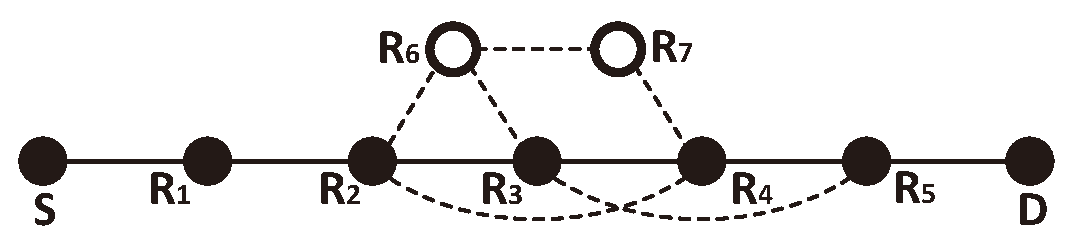
\includegraphics[width=7cm]{visio/attackmodel3.eps}
\caption{Adversary model where \emph{R}$_\emph{2}$ is the misbehaved entity and the purposed forwarding path is $\Psi$ \emph{=} $\langle$\emph{R}$_\emph{1}$\emph{, R}$_\emph{2}$\emph{, R}$_\emph{3}$\emph{, R}$_\emph{4}$\emph{, R}$_\emph{5}\rangle$ between {\tt S} and {\tt D}.}\label{attackmodel}
\end{center}
\vspace{-3mm}
\end{figure}
\vspace{-0.1in}
\subsection{Adversary Model}
In this paper, we focus on fault localization by performing packet delivery verification, which ensures source authenticity and correct packet forwarding. Intuitively, Fig. \ref{attackmodel} shows  examples of attacks. We assume \emph{R}$_\emph{2}$ is the misbehaved entity. and $\Psi$ \emph{=} $\langle$\emph{R}$_\emph{1}$\emph{, R}$_\emph{2}$\emph{, R}$_\emph{3}$\emph{, R}$_\emph{4}$\emph{, R}$_\emph{5}\rangle$, where $\Psi$ is the desired forwarding path. In this case, \emph{R}$_\emph{2}$ can modify the source address of IP packets originating from {\tt S} for launching \textbf{source spoofing} attack. Besides, \emph{R}$_\emph{2}$ can make the packets delivered along a path that differs from $\Psi$, e.g., $\langle$\emph{R}$_\emph{2}$\emph{, R}$_\emph{6}$\emph{, R}$_\emph{3}$$\rangle$, $\langle$\emph{R}$_\emph{2}$\emph{, R}$_\emph{6}$\emph{, R}$_\emph{7}$\emph{, R}$_\emph{4}$$\rangle$ and $\langle$\emph{R}$_\emph{2}$\emph{, R}$_\emph{4}\rangle$ for the purpose of \textbf{path inconsistency}\footnote{Traffic hijacking is one of the instantiations of forwarding path inconsistency attack.} attack. Moreover, if more than one misbehaved entities occur on $\Psi$, the packets can be transmitted along the unordered entities, e.g., $\langle$\emph{R}$_\emph{2}$\emph{, R}$_\emph{4}$\emph{, R}$_\emph{3}$\emph{, R}$_\emph{5}\rangle$.

As packets may be forwarded on unreliable communication channels, in particular, adversaries may interfere with fault localization, it is difficult to identify misbehaved entities. %localizing the misbehaved entity can be interfered if any fault occurs.}
%During the packet forwarding verification, localizing the misbehaved entity is a higher requirement if any error occurs. However, 
%In this case, 
The misbehaved entity can launch various \textbf{sophisticated attacks} to evade to be localized. In details, the attacks can be classified into two categories.
Firstly, the misbehaved entity can destroy or disturb fault localization by unexpectedly discarding, modifying and redirecting some messages used to localize the fault. For example, when {\tt S} tries to establish symmetric keys with intermediate entities on $\Psi$, \emph{R}$_\emph{2}$ can drop \emph{request} packets (from {\tt S} to \emph{R}$_\emph{i}$) or \emph{ack} packets (from \emph{R}$_\emph{i}$ to {\tt S}) to destroy this procedure of key distribution; or when \emph{R}$_\emph{3}$ reports \emph{ack} packet to {\tt S}, \emph{R}$_\emph{2}$ can modify this packet data to disturb the fault localization.
Secondly, the misbehaved entity can frame benign entities of their unrealistic misbehavior by launching frame attack. For example, when receiving a packet, \emph{R}$_\emph{2}$ greatly reduces the TTL value to 2, causing the illusion that \emph{R}$_\emph{4}$ is regarded as the fault due to its dropping the packet.
\vspace{-0.1in}
\subsection{Design Goal}
\label{desiredproperties}
To defend against the above adversary model, the following desired properties should be satisfied in fault localization. 

\noindent\textbf{Source and path verification.} Each entity on $\Psi$ can perform source and path verification. Once source spoofing or path inconsistency occurs, the entity can identify and filter the unreliable packets. 

%Note that, end-to-end communication sessions can be divided into consecutive \textbf{\emph{epochs}} that vary in different sessions and their phases. We perform the verification during each epoch. In one session, after {\tt S} sends an amount of packets to {\tt D} or a period of time interval expires, the \emph{epoch} value would be updated. 
\noindent\textbf{High accuracy of fault localization.} The source can effectively localize the fault with a high localization accuracy if any error occurs during symmetric key establishment or date forwarding verification. 

\noindent\textbf{Robustness and lightweight.} The fault localization can be robust and anti-attack, which no longer relies on reliable communication channels. Each entity is expectedly lightweight that does not store the symmetric keys shared with other network entities.
%\subsection{Problem Formulation}
%\label{problemformulation}
%This paper focuses on the data-plane fault localization for source authenticity and path compliance. 
%\textcolor{red}{In order to achieve fault localization, we formulate the several problems as the following definition shows.}\\
%\noindent{\textbf{Definition 1.}} We divide the end-to-end communication session into consecutive \textbf{\emph{epoch}}s, which varies with different sessions and their phases. For one session, after a period of time interval or {\tt S} sends an amount of packets to {\tt D}, the \emph{epoch} value would be switched.\\
%\noindent{\textbf{Definition 2.}} The \textbf{\emph{timer}} $\mathcal{T}_\emph{S}$ and $\mathcal{T}_\emph{i}$ are running on {\tt S} and \emph{R}$_\emph{i}$ on $\Psi$, respectively. They starts when the request package arrives and expires after a certain timeout, called \emph{\textbf{timer threshold}} that can be evaluated by a \emph{round-trip time} (RTT).\\ %of the corresponding entity on \emph{Path}$^\emph{*}$.\\
%\noindent{\textbf{Definition 3.}} In this paper, we denote \textbf{\emph{fault localization}} as to localize the misbehaved entity as well as its one neighbor, because accurately localizing the misbehaved entity is impossible to achieve according to the research \cite{barak2008protocols}. Of course, for the higher requirements, centralization-based mechanisms (e.g., VeriDP \cite{zhang2016mind}) in SDN, can be employed, which is not suitable for end-to-end communication.\\
%\noindent{\textbf{Definition 4.}} We define \emph{\textbf{positive ratio}} denoted by $\mathcal{P}_\emph{i}$ and $\mathcal{P}_\emph{D}$ for \emph{R}$_\emph{i}$ and {\tt D}, which illustrates the probability that the corresponding entity is misbehaved. When $\mathcal{P}_\emph{i}$ is larger than \emph{\textbf{positive ratio threshold}} (denoted by $\zeta$), and $\mathcal{P}_\emph{1}$, $\cdots$, $\mathcal{P}_{\emph{i-}1}$ are all less than $\zeta$, we can identify \emph{R}$_\tau$ or \emph{R}$_{\emph{i-}1}$ as the misbehaved entity (detailed in Section \ref{faultlocalization}).
%\vspace{-0.1in}

%In this paper, we focus on \textbf{\emph{fault localization}} as to localize misbehaved entities as well as its  neighbor, 
In this paper, we focus on the data-plane fault localization by verifying source authenticity and path consistency. We treat the detected entity and its neighbor as misbehaved entities because it is impossible to achieve the accuracy to a concrete entity of fault localization as the research \cite{barak2008protocols} describes. 
%Of course, for the higher requirements, centralization-based mechanisms (e.g., VeriDP \cite{zhang2016mind}) in SDN, can be employed, which is not suitable for end-to-end communication.\\
%\subsection{Scope and Assumptions}
%In this paper, we focus on the data-plane fault localization by verifying source authenticity and path consistency.  %while the packet is intended to be delivered through $\Psi$, 
We assume end hosts ({\tt S} and {\tt D}) are trusted because it is meaningless for a malicious source to detect faked packet source and wrong forwarding path. %As we perform data-plane detection, we assume 
Also, {\tt S} should know the packet forwarding path $\Psi$, which can be learned by the existing control-data plane routing protocols \cite{hu2004spv} \cite{murphy1996digital}, or it can be achieved by source routing \cite{sourcerouting}. %Due to the majority of symmetric forwarding path in today's Internet \cite{john2010estimating}, we assume \emph{Path}$^\emph{*}$ is symmetric.
%As for the secret key distribution, we assume the public/private key of 
Meanwhile, each entity on $\Psi$ has long-lived public and private keys, and the public keys can be retrieved and verified by others, which is similar to existing secure routing protocols~\cite{kim2014lightweight} \cite{basescu2016high} \cite{zhang2012shortmac} . 
%In this paper, we employ Dynamically Recreatable Key (DRKey) protocol \cite{kim2014lightweight} to establishes symmetric keys shared between routers and endhosts, in which routers don't need to store the keys that prevents state exhaustion DoS attacks.
%Due to the possible existence of malicious router(s), we assume any attacks can be launched to prevent the data-plane source and path monitoring. For example, the misbehaved router can disturb the symmetric key creation and distribution, and obstruct transmission of acknowledgements from kind nodes. 
%\vspace{-0.1in}
\section{Overview of \name{}}
\label{spmoniprotocoloverview}
We now describe the overview of the \name{} protocol that localizes faults even on unreliable transmission channels, e.g., in the presence of interference from adversaries. %achieve robust and lightweight fault localization for source authenticity and path compliance. Fig. \ref{workflow} depicts the work flow of RLFL protocol, which contains three phases with different purposes, as described blow.
%\subsection{High-Level Steps}
%\label{highlevelsteps}
Note that, in \name{}, end-to-end communication sessions are divided into consecutive \emph{epochs} that vary with different sessions and their phases of the sessions. In one session, after {\tt S} sends a number of packets to {\tt D} or a period of time interval expires, the \emph{epoch} value will be updated. \name{} performs the verification during each epoch. 

Fig. \ref{workflow} shows the workflow of \name{} protocol. At the beginning, \name{} enables the source {\tt S} to establish symmetric keys with all the other entities on $\Psi$.  
Using the symmetric keys, the packets verification and fault localization will then be carried out. Concretely, before each packet's departure, {\tt S} firstly inserts and initializes \name{} packets. Each entity will verify and probabilistically sample the packets on receiving them. At the end of each epoch, {\tt S} will perform fault localization according to the sampling information of entities.
\begin{figure}%[H]
\begin{center}
  % Requires \usepackage{graphicx}
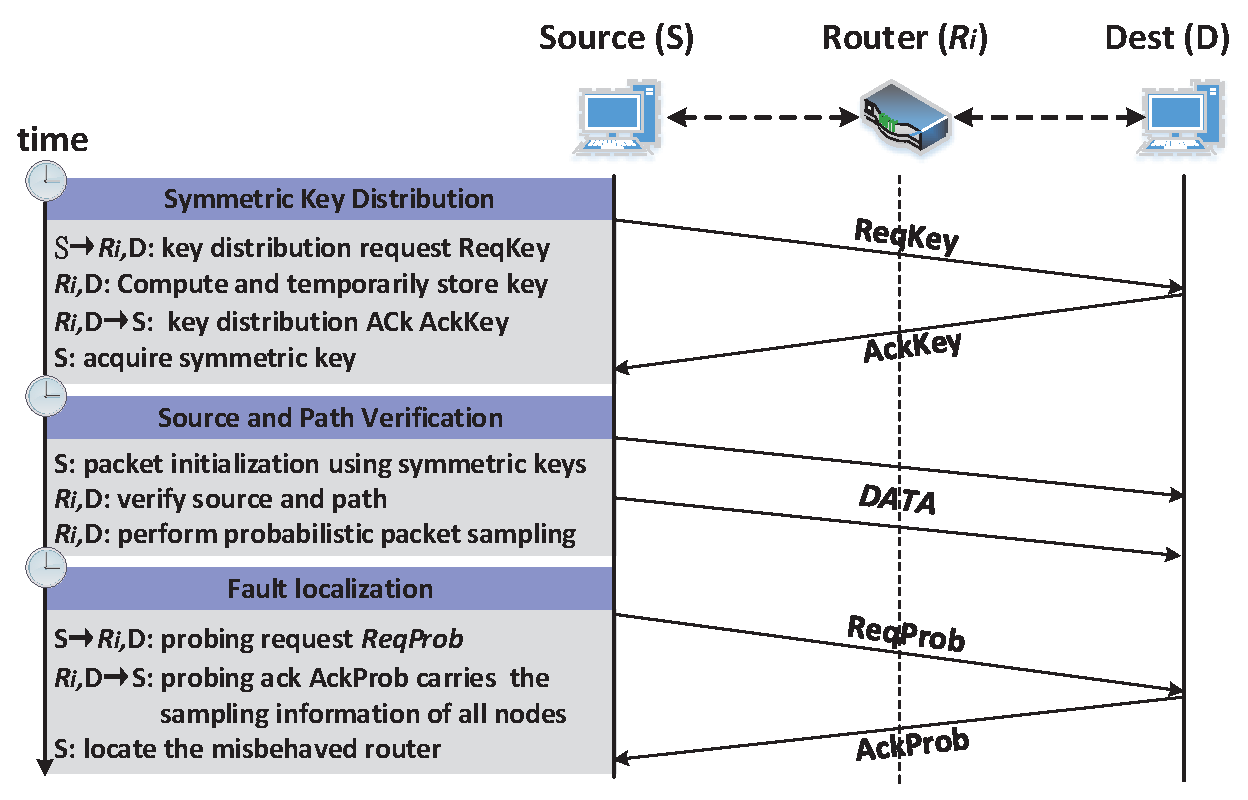
\includegraphics[width=8cm]{visio/workflow7.eps}
\caption{The workflow of \name{} protocol for the source ({\tt S}), intermediate entities (\emph{R}$_\emph{i}$) and the destination ({\tt D}), where ReqKey and AckKey (ReqProb and AckProb) respectively denote the request and acknowledgment messages for secret key distribution (fault localization) probing.}\label{workflow}
\end{center}
\vspace{-3mm}
\end{figure}\\
%RFL allows these entities to sign and verify packet information by using the keys such that it localizes faults.\\
%\noindent{\textbf{Symmetric key distribution.}} We propose a lightweight and anti-attack symmetric key distribution protocol called \emph{LASKey} to guarantee secure key distribution. As shown in Fig. \ref{workflow}, \emph{S} sends a request packet (denoted by ReqKey) along \emph{Path}$^\emph{*}$ towards \emph{D}. Each entity computes and temporarily store the symmetric key. Upon receiving the message, \emph{D} initializes and sends an ack packet (denoted by AckKey) back to \emph{S}, which would carry the encrypted symmetric key of each hop in the path and the signatures of these entities on reversed \emph{Path}$^\emph{*}$.
%Concretely, \emph{D} initializes and adds its encrypted \emph{K}$_{\emph{S,D}}$ to \emph{AckKey} packet; each router \emph{R}$_\emph{i}$ inserts its encrypted \emph{R}$_{\emph{S,R}_\emph{i}}$ and signatures into \emph{AckKey} packet before $\mathcal{T}_\emph{i}$ expires.
%Based on the received AckKey packet, \emph{S} decrypts and obtains the symmetric keys.\\
\noindent{\textbf{Robust symmetric key distribution.}}
\name{} introduce a robust symmetric key distribution called \namekey{} to guarantee secure key establishment and allocation between {\tt S} and network entities in forwarding path. As shown in Fig. \ref{workflow}, {\tt S} sends a request packet (denoted by ReqKey) along $\Psi$ towards {\tt D}. Each entity computes and temporarily store the symmetric key. Upon receiving ReqKey, {\tt D} initializes and sends an ack packet (denoted by AckKey) back to {\tt S}, which will gradually record the encrypted symmetric keys and signatures of each entity on $\Psi$ hop by hop during AckKey's delivery to {\tt S}.
Based on the received AckKey, {\tt S} decrypts and obtains the symmetric keys.\\
\noindent{\textbf{Lightweight source and path verification.}}
After obtaining the symmetric keys, {\tt S} precomputes a marking for each entity on $\Psi$ before sending out a data packet. All markings are inserted into a new header called \name{} header between IP header and TCP header.
During the packet transmission, each entity \emph{R}$_\emph{i}$ performs packet forwarding verification by recalculating its own marking using symmetric key \emph{K}$_{\emph{S,R}_\emph{i}}$ once receiving packets, and comparing it with the inserted one on \name{} header. Only these two values are equal, can \emph{R}$_\emph{i}$ forward the packet to downstream entities. Note that each intermediate entity \emph{R}$_\emph{i}$ does not require to store symmetric keys for each flow, which introduces the lightweight \name{} router.\\
%Note that the source address and the destination address is used as the input to compute each node's marking, which could defense source spoofing and traffic redirection. The address of one-hop upstream router as one input of marking computation prevent the forwarding path from deviation. Besides, marking calculation also employs TTL value and all downstream routers' markings to defense against frame attacks, such as TTL attack.
\noindent{\textbf{Robust fault localization.}}
\name{} enables entities to sample packets for fault localization. {\tt S} uses the packet sampling information of each entity on $\Psi$ to localize the fault. Our developed probabilistic packet sampling function $\mathcal{F}$ (described in Section \ref{faultlocalization}) determines which entity will sample the packet in one epoch. Each entity's packet sampling results can be only predicted by {\tt S}, but unknowable to others. Concretely, {\tt S} uses $\mathcal{F}$ to learn which entities will sample a packet. Upon receiving the packet, the entities (\emph{R}$_\emph{i}$ and {\tt D}) perform $\mathcal{F}$ to sample the packet and store the results in a bloom filter. At the end of each epoch, {\tt S} sends a request probing packet, called ReqProb, to ask all entities on $\Psi$ for their sampling information of this epoch. The ack message (denoted by AckProb) carrying the encrypted sampling information will be delivered from {\tt D} to {\tt S}.
Thereby, based on the received AckProb, {\tt S} determines where a fault occurs (detailed in Section \ref{faultlocalization}).\\
\indent
However, %\textcolor{red}{since the unreliable communication channels can tolerate corrupting fault localization,} 
it is challenging to implement \name{} because of the following issues:\\
\noindent \textbf{Corrupting symmetric key distribution.} The symmetric key is the important guarantee to correctly perform packet forwarding verification and fault localization. If the adversary maliciously corrupts symmetric key distribution (e.g., modify, drop and redirect the ReqKey or AckKey). \name{} will become paralyzed and unable to localize the fault. Meanwhile, if each entity needs to store one symmetric key per-session, the state exhaustion (e.g., DoS)  attacks will be easier to happen, which is infeasible in the practical networks.\\
\noindent{\textbf{Unreliable packet transmission.}} The adversary can destroy the transmission of request or ack packet for corrupting \name{}. When {\tt S} sends request packets (ReqKey and ReqProb), the misbehaved entity can drop or redirect these packets to disturb symmetric key distribution or {\tt S}'s obtaining sampling information. Thereby, any entity can not reply its symmetric key or packet sampling result back to {\tt S}, incurring the failure of fault localization. Also, the entity can modify the data of ack packets (AckKey and AckProb). Even though {\tt S} can capture the modified data by checking signatures on these ack packets, it can not identify and localize the fault.\\
\noindent{\textbf{Interference by frame attacks.}} The misbehaved entity can launch frame attacks to corrupt \name{}. This can try to make benign entities mistakenly perform packet forwarding verification, which can frame them for destroying reliable packet delivery. For example, TTL attack can be used to significantly decrease TTL value of any packets so as to frame the benign entity of dropping packets. Moreover, when performing source and path verification, the misbehaved entity can tamper the pre-inserted markings in \name{} header, resulting in the verification failure or packets discard to disturb the fault localization.
%In \name{} protocol, \emph{S} uses the packet sampling information of each node on \emph{Path}$^\emph{*}$ to determine the location of the fault. Our proposed probabilistic packet sampling function $\mathcal{F}$ (described in Section \ref{faultlocalization}) determines whether the current packet would be sampled at \emph{R}$_\emph{i}$ or \emph{D}. Each node's packet sampling results can be predictable by \emph{S}, but unknowable to other nodes.
%Before each packet's departure, \emph{S} uses $\mathcal{F}$ to learn which node(s) would sample this packet. When receiving the packet, \emph{R}$_\emph{i}$ and \emph{D} perform $\mathcal{F}$ to sample the packet and store it in a bloom filter. At the end of each epoch, \emph{S} send a request probing packet, called \emph{ReqProb}, to ask all nodes on \emph{Path}$^\emph{*}$ for their sampling information of this epoch. Then the ack probing packet called \emph{AckProb} is forwarded from \emph{D} to \emph{S}. When AckProb packet reaches each hop on \emph{Path}$^\emph{*}$, each node would add its own encrypted sampling information to AckProb. %Note that \emph{R}$_\emph{i}$ would send its own sampling information \emph{AckProb}$_\emph{i}$ back to \emph{S} when $\mathcal{T}_\emph{i}$ expires, as Section \ref{askeymechanismovervies} describes.
%Based on the received AckProb, \emph{S} determines the fault location according to the difference between the received sampling information and the predicted one of each node.
%We lower the storage overhead of each node by reducing the bloom filter length in the following ways: (i) the session is divided into consecutive epoches, enabling each node not have to sample all packets of the session; (ii) $\mathcal{F}$ provides probabilistic packet sampling, enabling each node not have to sample all packets of each epoch. Considering the transmission delay, two bloom filters for each node on \emph{Path}$^\emph{*}$ should be established and stored by \emph{S}, one for the current epoch and another for the next epoch. Meanwhile, each node also builds two bloom filters for the current and the next epoch. If the sampling information of one epoch is reported to \emph{S} and employed, the corresponding bloom filter would be emptied for the continuous usage.
%\subsection{Challenges in \name{} protocol}
%\label{challengesoverview}
%Based on the high-level description, \name{} protocol faces serious security vulnerabilities, especially in unreliable transmission channel, which allows the misbehaving router to disturb any form of fault localization.\\
%\noindent{\textbf{Disturbing the transmission of request and ack packet.}} When \emph{S} sends request packet ReqKey and ReqProb, the misbehaving router could drop or redirect these packet to disturb symmetric key distribution or fault localization. Unreceiving request packets, entities would not send their encrypted symmetric key or packet sampling information back to \emph{S}, causing the failure of fault localization. In addition to dropping or redirecting, the offending router could also modify the packet data of AckKey and AckProb. Even though knowing the packet data has already been maliciously modified checking signatures, \emph{S} could not identify and localize the fault.\\
%\noindent{\textbf{Launching the frame attacks to blame others.}} To evade to be localized, the misbehaving router could launch TTL attack by greatly decreasing TTL value of any received packets for framing other entities. Besides, when performing source and path verification, the misbehaving entity could modify the pre-inserted markings in \name{} header, causing the failure of verification, and packet dropping by other router, which disturbs the fault localization accuracy.

%\subsection{Lightweight and Anti-attack Key Distribution}
%\label{askeymechanismovervies}
%At the beginning of RLFL protocol, symmetric keys shared between \emph{S} and each node on \emph{Path}$^\emph{*}$ is established and distributed. We propose a lightweight and anti-attack symmetric key distribution mechanism, called \emph{LASKey}, to guarantee the security of key distribution. LASKey mechanism provides two vital properties. (i) Lightweight: each router do not have to store the symmetric key, regardless of the number of flows and sources. (ii) Anti-attack: \emph{S} could locate the misbehaved router who disturbs or destroys LASKey mechanism, which offers the robustness for symmetric key distribution.

%Consider the scenario of Fig. \ref{attackmodel}.
%When establishing symmetric keys, \emph{S} firstly sends request packet (denoted by \emph{ReqKey}) along \emph{Path}$^\emph{*}$ towards \emph{D}. Each router \emph{R}$_\emph{i}$ computes \emph{K}$_{\emph{S,R}_\emph{i}}$ and start the timer $\mathcal{T}_\emph{i}$ on receiving \emph{ReqKey} packet. When \emph{ReqKey} packet arrives at \emph{D}, the acknowledgment packet (denoted by \emph{AckKey}) is forwarded towards \emph{S}, which carries the encrypted symmetric keys and signatures of all nodes on reversed \emph{Path}$^\emph{*}$. Concretely, \emph{D} initializes and adds its encrypted \emph{K}$_{\emph{S,D}}$ to \emph{AckKey} packet; each router \emph{R}$_\emph{i}$ inserts its encrypted \emph{R}$_{\emph{S,R}_\emph{i}}$ and signatures into \emph{AckKey} packet before $\mathcal{T}_\emph{i}$ expires. Based on the received \emph{AckKey} packet, \emph{S} performs decryptions and obtains the symmetric keys.

%Note that all nodes on \emph{Path}$^\emph{*}$ would check the authenticity of \emph{ReqKey} and \emph{AckKey} packets by verifying the signatures when receiving these two packets. Due that the misbehaved router might modify, drop and redirect \emph{ReqKey} or \emph{AckKey} packet, \emph{R}$_\emph{i}$ might not receive \emph{AckKey} within timer threshold. In this case, \emph{R}$_\emph{i}$ initializes and sends \emph{AckKey}$_\emph{i}$ towards \emph{S}. \emph{R}$_{\emph{i-}1}$, $\cdots$, \emph{R}$_\emph{1}$ add their encrypted symmetric keys and signatures to \emph{AckKey}$_\emph{i}$. In this case, \emph{S} decrypts \emph{AckKey}$_\emph{i}$ instead of \emph{AckKey} packet, only obtaining \emph{K}$_{\emph{S,R}_1}$, $\cdots$, \emph{K}$_{\emph{S,R}_\emph{i}}$. This help to locate $\langle$\emph{R}$_\emph{i}$\emph{,R}$_{\emph{i+}1}$$\rangle$ as the fault.

%\subsection{Source and Path Verification}
%In order to achieve the source and path validation at each hop and prevent the destination from exhaustion, \emph{S} precomputes the marking for each node on \emph{Path}$^\emph{*}$ using the obtained symmetric key. These markings are all inserted into RLFL header, which is added between IP header and TCP/UDP header of IP packet. Once receiving the packet, \emph{R}$_\emph{i}$ recalculates its marking using \emph{K}$_{\emph{S,R}_\emph{i}}$ and compares it with the one on RLFL header. Only these two values is consistent, can \emph{R}$_\emph{i}$ forward the packet to downstream routers.

%Note that the source address and the destination address is used as the input to compute each node's marking, which could defense source spoofing and traffic redirection. The address of one-hop upstream router as one input of marking computation prevent the forwarding path from deviation. Besides, marking calculation also employs TTL value and all downstream routers' markings to defense against frame attacks, such as TTL attack. 
\vspace{-0.1in}
\section{Robust Symmetric Key Distribution}
\label{lakeysection}
%\textcolor{red}{
In this section, we present our proposed \namekey{}, a robust symmetric key sharing between {\tt S} and each entity on $\Psi$, which allows different entities to obtain correct keys so that it can perform correct localization. % of \name{}. %\namekey{} is well employed to achieve shared keys setup and distribution in the initial period of \name{}, which promotes the robustness of fault localization for source and path verification.} 
Similar to DRKey \cite{kim2014lightweight}, \namekey{} provides the stateless operation on routers and enables each router not to store the symmetric keys. More especially, it also offers robustness against the interference of misbehaving entities. Fig. \ref{askeyfigure} shows how \namekey{} works when each entity creates the symmetric key and shares it with {\tt S}.
\vspace{-0.1in}
\subsection{ReqKey transmission from {\tt S} to {\tt D}}
\label{reqkeytransmission}
\begin{figure}%[H]
\begin{center}
  % Requires \usepackage{graphicx}
\includegraphics[width=8.3cm]{visio/laskey3.eps}
\caption{\namekey{} for symmetric key distribution with $\Psi$\emph{=}$\langle$\emph{S, R}$_1$\emph{,}$\cdots$\emph{R}$_\emph{n}$\emph{, D}$\rangle$, where \emph{R}$_{\emph{n+}1}$ is regarded as the destination {\tt D}.}\label{askeyfigure}
\end{center}
\vspace{-3mm}
\end{figure}
To achieve sharing symmetric keys with other entities, {\tt S} initializes ReqKey packet and %, which is then forwarded 
delivers it to {\tt D} through $\Psi$.
%At the beginning, ReqKey packet is firstly initialized by {\tt S} and then forwarded through $\Psi$ to {\tt D}. 
ReqKey contains $\Psi$, session identifier \emph{SessionID}, the public key set \emph{PubK} of all entities on $\Psi$ and {\tt S}'s signature \emph{Sign}$_\emph{S}$, as Eq. \ref{reqkeyfomat} shows.
\begin{equation}\label{reqkeyfomat}
\emph{ReqKey} =~ \{\Psi, \emph{SessionID}, \emph{PubK}, \emph{Sign}_\emph{S}\},
%\vspace{-0.06in}
\end{equation}
\noindent where \emph{SessionID} is the session identifier that is the hash over end-hosts' public keys (\emph{K}$_\emph{S}$ and \emph{K}$_\emph{D}$) and session's start time \emph{T}$_\emph{start}$. It can be computed by the following equation:
\begin{equation}\label{sessionidkey}
\emph{SessionID} = H(\emph{K}_\emph{S}\vert \vert \emph{K}_\emph{D}\vert \vert \emph{T}_{\emph{start}}).
\end{equation}
As Eq. \ref{signaturesource} shows, \emph{Sign}$_\emph{S}$ uses the destination address ({\tt D}) as one of the inputs, contributing to defending against ReqKey redirection or hijacking by modifying the destination address of ReqKey packet. %For example, if a misbehaved router redirects or hijacks \emph{ReqKey}, the downstream routers can drop this packet as the failed verification for \emph{Sign}$_\emph{S}$.
Certainly, \emph{Sign}$_\emph{S}$ is also keyed with \emph{K}$_\emph{S}^{\emph{-}1}$ that makes ReqKey away from source spoofing.
\begin{equation}\label{signaturesource}
\emph{Sign}_\emph{S} = \emph{Sign}_{\emph{K}^{\emph{-}1}_\emph{S}}H({\tt D}\vert \vert \Psi \vert \vert \emph{SessionID} \vert \vert \emph{PubK}).
\end{equation}

In addition to checking \emph{Sign}$_{\emph{S}}$, each intermediate entity \emph{R}$_\emph{i}$ creates and temporarily stores the symmetric key \emph{K}$_{\emph{S,R}_\emph{i}}$, which is calculated using pseudo-random function (PRF) keyed by local secret information (\emph{LSI}$_\emph{i}$), only known by \emph{R}$_\emph{i}$ (see Eq. \ref{ksri}).
\begin{equation}\label{ksri}
\emph{K}_{\emph{S}, \emph{R}_\emph{i}} = \emph{PRF}_{\emph{LSI}_\emph{i}}(\emph{SessionID} \vert \vert {\tt S}).
\end{equation}
\emph{R}$_\emph{i}$ starts the timer $\mathcal{T}_\emph{i}$ when ReqKey is delivered to the downstream entity, where $\mathcal{T}_\emph{i}$ is the timer maintained on \emph{R}$_\emph{i}$. 
%The \textbf{\emph{timer}} $\mathcal{T}_\emph{S}$ and $\mathcal{T}_\emph{i}$ are running on {\tt S} and \emph{R}$_\emph{i}$ on $\Psi$, respectively. 
It starts when the request package arrives and expires after a certain timeout, called \emph{\textbf{timer threshold}} that can be obtained by a \emph{round-trip time} (RTT). 
 %, and the temporary storage time of \emph{K}$_{\emph{S,R}_\emph{i}}$ relies on timer threshold. Unlike DRKey, our proposed \emph{LASKey} enable each router not have to insert the encrypted key into request packet, avoiding the risk of modification, discarding and redirection of the encrypted keys. Instead,
The created key \emph{K}$_{\emph{S,R}_\emph{i}}$ is temporarily stored until AckKey (detailed shortly) comes or $\mathcal{T}_\emph{i}$ expires. More considerately, \namekey{} makes each entity temporarily record the TTL value \emph{ttl}$_\emph{i}^\emph{r}$ of received ReqKey, which helps to avoid TTL attack.
\vspace{-0.1in}
\subsection{AckKey Transmission from {\tt D} to {\tt S}}
\label{ackkeytransmission}
To reply ReqKey, AckKey is initialized by {\tt D} and then sent back through intermediate entities towards {\tt S}, whose construction is as Eq. \ref{ackkeyformat} shows.
\begin{equation}\label{ackkeyformat}
\emph{AckKey} =~ \{\emph{ReqKey}, \emph{EncK}_{\emph{S,D}}, \emph{SignK}_\emph{D}\}.
%\vspace{-0.06in}
\end{equation}
\noindent
$\emph{EncK}_{\emph{S,D}}$ and $\emph{SignK}_\emph{D}$ are the encrypted \emph{K}$_{\emph{S},\emph{D}}$ and {\tt D}'s signature, respectively (detailed in Fig. \ref{askeyfigure}).\\
\indent
During AckKey's transmission, each entity adds its encrypted symmetric key \emph{EncK}$_{\emph{S,R}_\emph{i}}$ and signature \emph{SignK}$_{\emph{R}_\emph{i}}$ into AckKey. Note that when computing the signature \emph{SignK}$_{\emph{R}_\emph{i}}$, the encrypted symmetric keys and signatures of downstream entities (i.e., \emph{R}$_{\emph{i+}1}$,$\cdots$,\emph{R}$_\emph{D}$) will also be added as the input. In this case, each router \emph{R}$_\emph{i}$ only checks the \emph{SignK}$_{\emph{R}_{\emph{i+}1}}$ of its 1-hop downstream \emph{R}$_{\emph{i+}1}$, which can also defend against frame attack. Therefore, AckKey has the following construction (Eq. \ref{ackkeyformati}) when it arrives at \emph{R}$_\emph{i}$:\\
\begin{equation}\label{ackkeyformati}
\emph{AckKey} =~ \{\emph{ReqKey}, \emph{EncKset}_{\emph{i}}, \emph{SignKset}_\emph{i}, \emph{SignK}_{\emph{S},\emph{R}_\emph{i}}\},
%\vspace{-0.06in}
\end{equation}
\noindent where \emph{EncKset}$_\emph{i}$ and \emph{SignKset}$_\emph{i}$ are the sets of encrypted symmetric keys and signatures, respectively. Thus, AckKey can record the encrypted symmetric keys of all entities when it arrives at {\tt S}, as case \uppercase\expandafter{\romannumeral1} in Fig. \ref{disburbacktransmission} shows.\\
\indent To deal with the malicious discarding of either ReqKey or AckKey packet by the misbehaved entity, each entity (including {\tt S}) starts the timer $\mathcal{T}_\emph{i}$ when ReqKey passes through. If $\mathcal{T}_\emph{i}$ expires, i.e., \emph{R}$_\emph{i}$ does not receive AckKey within timer threshold, \emph{R}$_\emph{i}$ initializes a new AckKey, which contains \emph{EncK}$_{\emph{S,K}_{\emph{R}_\emph{i}}}$ and \emph{Sign}$_{\emph{K}_{\emph{R}_\emph{i}}}$. Thus, if any misbehaved entity drops ReqKey or AckKey, its upstream entity close to {\tt S} will forward their encrypted keys and signatures to {\tt S}. This is as case \uppercase\expandafter{\romannumeral2} in Fig. \ref{disburbacktransmission} shows, where the misbehaved entity \emph{R}$_\emph{3}$ can modify, drop and redirect ReqKey or AckKey packet for disturbing {\tt S}'s obtaining all entities' sampling information.
In this case, {\tt S} can achieve the fault localization to identify the misbehaved entity (described shortly). To avoid TTL attack, we use TTL values of both received ReqKey and AckKey as the input to compute \emph{SignK}$_{\emph{R}_\emph{i}}$. When AckKey is verified at each hop, \emph{R}$_\emph{i}$ obtains purposed TTL value of ReqKey and AckKey of other entities based on $\Psi$, and then use them to check others' signatures. If the misbehaved entity launches TTL attack, the signatures of its downstream entities will not be verified successfully.
%In \emph{LASKey} mechanism, a timer $\mathcal{T}$ is established on each node, which can defend against the discarding of \emph{ReqKey} and \emph{AckKey}. If the misbehaved router (say, \emph{R}$_\tau$) drops \emph{ReqKey} and \emph{AckKey} to disturb symmetric key distribution, the timer $\mathcal{T}_{\tau\emph{-}1}$ of its upstream router \emph{R}$_{\tau\emph{-}1}$ will expires, resulting in the transmission of its encrypted symmetric key and signature back to \emph{S}. Thus, if the discarding of \emph{ReqKey} or \emph{AckKey} occurs, \emph{S} can locate the misbehaved node according to the received \emph{AckKey} packet.
\begin{figure}%[H]
\begin{center}
  % Requires \usepackage{graphicx}
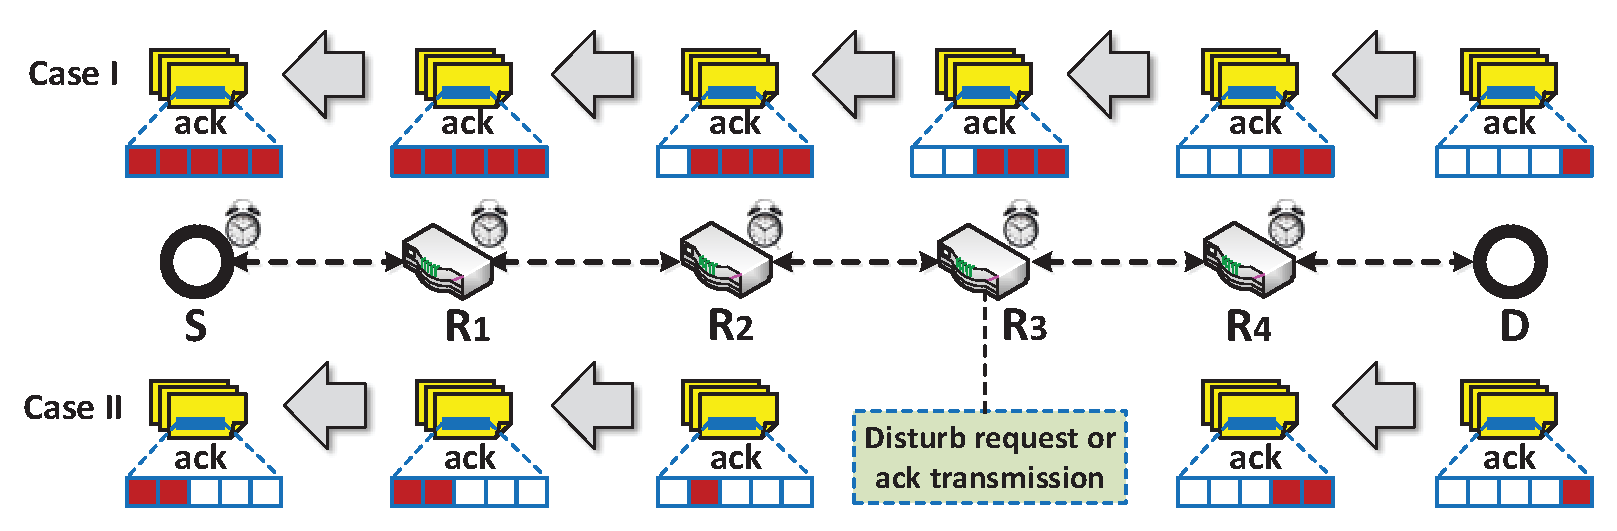
\includegraphics[width=1\columnwidth]{visio/disturbacktransmission.eps}
\caption{\namekey{} can ensure the robustness of symmetric keys distribution even facing unreliable communication channels. The red rectangle represents the ack of each network entity. Case \uppercase\expandafter{\romannumeral1} shows the AckKey packet can be securely delivered to {\tt S}, while case \uppercase\expandafter{\romannumeral2} depicts the misbehaved entity \emph{R}$_\emph{3}$ can interfere with ReqKey or AckKey packet transmission.}\label{disburbacktransmission}
\end{center}
\vspace{-3mm}
\end{figure}
\vspace{-0.1in}
\subsection{Symmetric Key Acquisition}
\label{keyacquisition}
The source {\tt S} needs to retrieve the symmetric keys shared with other entities on $\Psi$, which can be used to perform packet forwarding verification and fault localization.
In \name{}, {\tt S} can obtain symmetric keys from the received AckKey packet. Concretely, once receiving the AckKey packet, {\tt S} firstly checks the signatures and decrypts the encrypted keys to obtain the symmetric keys. Concretely, for each entity from \emph{R}$_1$ to {\tt D} on $\Psi$, if its signature is verified successfully using its public key, {\tt S} can obtain the symmetric key by decrypting the encrypted key using {\tt S}'s private key. In this way, the symmetric key set (denoted by $\mathbb{L}$) can be obtained:
\begin{equation}\label{symmetrickeyset}
\mathbb{L} ~\emph{=} ~\left \langle \emph{K}_{\emph{S},\emph{R}_1}, \emph{K}_{\emph{S},\emph{R}_2}, \cdots, \emph{K}_{\emph{S},\emph{D}} \right \rangle.
%\vspace{-0.06in}
\end{equation}
\indent Obviously, as there may be misbehaved entities to disturb the transmission of ReqKey and AckKey, {\tt S} may only gain the subset (denoted by $\mathbb{L}^{\prime}$) of $\mathbb{L}$, i.e., $\mathbb{L}^{\prime}\subseteq\mathbb{L}$:
\begin{equation}\label{symmetrickeyset1}
\mathbb{L}^\prime ~\emph{=} ~\left \langle \emph{K}_{\emph{S},\emph{R}_1}, \emph{K}_{\emph{S},\emph{R}_2}, \cdots, \emph{K}_{\emph{S},\emph{R}_\emph{m}} \right \rangle.
%\vspace{-0.06in}
\end{equation}
Then {\tt S} affirms confidently there is at least one misbehaved entity between \emph{R}$_\emph{m}$ and \emph{R}$_{\emph{m+}1}$ on $\Psi$. Another case is that {\tt S} never receives AckKey or AckKey$_\emph{i}$ before the timer maintained in $S$, i.e., $\mathcal{T}_\emph{S}$, expires, which illustrates \emph{R}$_1$ did not initialize and send AckKey$_1$ back. In this case, \emph{R}$_1$ will be localized as the fault. With the function of fault localization, our proposed \namekey{} provides more secure symmetric key distribution, where the misbehaved entity has to behave normally to avoid to be localized as the fault. 
%\vspace{-0.1in}
\section{Lightweight Source and Path Verification}
\label{sourceandpathverificationsection}
In this section, we detailedly describe the design details of source and path verification. \name{} enables {\tt S} to initialize the \name{} protocol and entities to perform the packet verification that is lightweight as no symmetric key need to stored. Concretely, {\tt S} uses the obtained symmetric keys to precompute the markings for each entity on $\Psi$ and inserts these markings into \name{} header, a new packet header between IP header and TCP header. During the packet delivery towards {\tt D}, each entity dynamically recomputes the secret key and then verifies the packet by recalculating the marking.
\vspace{-0.1in}
\subsection{\name{} Protocol Initialization}
\label{spmoniheaderinitialization}
\name{} protocol is initialized to make the markings for each entity calculated and inserted in packet header. \name{} enables {\tt S} to compute the markings using symmetric keys for all entities, and generates a new packet header called \name{} header to include the marking information, which is embedded between IP header and TCP header. Before sending out packets, {\tt S} initializes \name{} headers with the following structure:
%\vspace{-0.06in}
\begin{equation}\label{spmoniheader}
\emph{\name{} header} =~ \{\emph{SessionID}, \emph{epoch}, \emph{PacketID}, \emph{M}_{\emph{Path}}\}.
%\vspace{-0.06in}
\end{equation}
\noindent \emph{PacketID} is the unique packet identifier, calculated based on Eq. \ref{packetid}:
%\vspace{-0.06in}
\begin{equation}\label{packetid}
\emph{PacketID = H}(\emph{SessionID} \vert \vert \emph{epoch} \vert \vert \emph{IP}_{\emph{cst}}),
%\vspace{-0.06in}
\end{equation}
\noindent where \emph{IP}$_{\emph{cst}}$ represents constant portion of IP packet (excluding variable fields, such as TTL and checksum) during forwarding. The \emph{M}$_{\emph{Path}}$ (in Eq. \ref{spmoniheader}) denotes the precomputed marking sequence for later verification at each entity, as Eq. \ref{mpath} shows.
%\vspace{-0.06in}
\begin{equation}\label{mpath}
    \emph{M}_{\emph{Path}} ~\emph{=}~ \left \langle \emph{M}_\emph{1}, \emph{M}_\emph{2}, \cdots, \emph{M}_\emph{n}, \emph{M}_\emph{\emph{\emph{D}}} \right \rangle,
%\vspace{-0.06in}
\end{equation}
where \emph{M}$_{\emph{i}}$ is precalculated for each entity using PRF keyed with the shared symmetric keys, as Eq. \ref{mid} shows, where \emph{M}$_{\emph{cst}}^{\emph{in}}$ is the splice of constant input: $\emph{SessionID} \vert \vert \emph{epoch} \vert \vert \emph{PacketID} \vert \vert \emph{S} \vert \vert \emph{D}$. Adding source and destination address (denoted by \emph{S} and \emph{D}) as the input can also help to defense against both source spoofing and traffic redirection, caused by modifying source and destination address of IP packet.\\
\indent In Eq. \ref{mid}, \emph{TTL}$_\emph{i}$ and \emph{TTL}$_\emph{D}$ respectively donates the purposed TTL value when the packet arrives at \emph{R}$_\emph{i}$ and {\tt D}. %\emph{R}$_{\emph{i-}1}$ (\emph{1}$\leq i \leq$\emph{n}) is one-hop upstream router's address of \emph{R}$_\emph{i}$ where \emph{R}$_{\emph{i-}1}$ \emph{= S} when \emph{i =} 1.
The marking is precomputed for the entity on the reverse $\Psi$. More especially, all downstream entities' markings are added as the input, which prevents frame attack caused by malicious modification of the pre-inserted markings of downstream entities.
\vspace{-0.06in}
\begin{equation}\label{mid}
    \begin{split}
    \emph{M}_\emph{D} &~\emph{=} ~\emph{PRF}_{\emph{K}_{\emph{S,D}}}(\emph{M}_{\emph{cst}}^{\emph{in}} \vert \vert \emph{TTL}_\emph{D} \vert \vert \emph{R}_\emph{n}).\\
%    \emph{M}_\emph{n} &~\emph{=} ~\emph{PRF}_{\emph{K}_{\emph{S,R$_\emph{\emph{n}}$}}}(\emph{M}_{\emph{cst}}^{\emph{in}}\vert \vert \emph{TTL}_{\emph{n-}1} \vert \vert \emph{R}_{\emph{n-}1} \vert \vert \emph{M}_\emph{D})\\
%    & \cdots\cdots \\
    \emph{M}_\emph{i} &~\emph{=} ~\emph{PRF}_{\emph{K}_{\emph{S,R$_\emph{\emph{i}}$}}}(\emph{M}_{\emph{cst}}^{\emph{in}} \vert \vert \emph{TTL}_\emph{i} \vert \vert \emph{R}_{\emph{i-}1} \vert \vert \emph{M}_{\emph{i+}1} \vert \vert \cdots \vert \vert \emph{M}_\emph{n} \vert \vert \emph{M}_\emph{D} ).\\
    \end{split}
\vspace{-0.06in}
\end{equation}
\indent The fields \emph{SessionID}, \emph{epoch} and \emph{PacketID} in \name{} header respectively occupies 128 bits, 16 bits and 128 bits. Each marking occupies 32 bits, whose rationality analysis is shown in Section \ref{theoreticalanalysis}.
\vspace{-0.1in}
\subsection{Source and Path Verification}
\label{sourceandpathverification}
\name{} allows each intermediate entity to verify packet source and forwarding path by verifying the markings encoded in the packets. Note that \name{} enables each entity on $\Psi$ not to store the symmetric key, which can be calculated according to Eq. \ref{ksri}. This makes entities lightweight and can protect the state of exhaustion (e.g., DoS) attack. After \name{} header initialization, each packet departs from {\tt S} and is delivered through intermediate routers towards {\tt D}. During the transmission, the packet is verified for its origin and forwarding path at each hop.
%\noindent{\textbf{Source and path verification.}}
Concretely, each entity uses Eq. \ref{mid} to recalculate the marking \emph{M}$_\emph{i}'$. If the computed \emph{M}$_\emph{i}'$ equals to \emph{M}$_\emph{i}$ in \name{} header, it illustrates that the source and the forwarding path are all correct up to the current entity. Else, i.e., the verification fails, the packet will is dropped at this hop. This verification by each entity for the received packet can prevent the state exhaustion attacks on {\tt D}. 
%\vspace{-0.1in}
\section{Robust Fault Localization}
\label{faultlocalization}
\begin{algorithm}[t]
\footnotesize
\caption{ReqProb and AckProb Initialization.}
\label{reqpketinitialization}
\begin{algorithmic}[1]
\Function {\emph{ReqProb} Initialization by {\tt S}~~} { }\\
    $\textbf{Require}$: $\Psi$, $\emph{SessionID}$, \emph{epoch}, \emph{S}, \emph{D}\\
    $\textbf{Compute}$:
    %\State $\xi_{\emph{max}}^\emph{e}$ ~\emph{=}~ \emph{max}~\{$\xi_\emph{1}^\emph{e}$, $\cdots$, $\xi_{\emph{n}}^\emph{e}$, $\xi_{\emph{D}}^\emph{e}$\}
    \State $\emph{M}_{\emph{cst}}^\emph{req}$ ~\emph{=}~ $\Psi\vert \vert$\emph{SessionID}$\vert \vert$\emph{epoch}$\vert \vert$\emph{S}$\vert \vert$\emph{D}
    %\If{$\xi_{\emph{max}}^\emph{e}$ $\geq$ $\xi_{\emph{th}}^\emph{e}$} \label{iii}
    \State $\emph{M}_\emph{D}^{\emph{req}}$ \emph{=} \emph{PRF}$_{\emph{K}_{\emph{S,D}}}$($\emph{M}_{\emph{cst}}^\emph{req}\vert \vert$\emph{TTL}$_\emph{D}\vert \vert$\emph{R}$_\emph{n}$)
    \For {\emph{i} from \emph{n} to 1}
    \State $\emph{M}_\emph{i}^{\emph{req}}$ \emph{=} \emph{PRF}$_{\emph{K}_{\emph{S,D}}}$($\emph{M}_{\emph{cst}}^\emph{req}\vert \vert$\emph{TTL}$_\emph{i}\vert \vert$\emph{R}$_{\emph{i}-1} \vert \vert$\emph{M}$_{{i}+1}^{\emph{req}} \vert \vert \cdots \vert \vert$\emph{M}$_\emph{n}^{\emph{req}}\vert \vert$\emph{M}$_\emph{D}^{\emph{req}}$)
    \EndFor
    \State \emph{M}$_\emph{Path}^\emph{req}$ \emph{ = } $\langle$\emph{M}$_1^\emph{req}$, $\cdots$, \emph{M}$_\emph{n}^\emph{req}$, \emph{M}$_\emph{D}^\emph{req}\rangle$
    \State \emph{ReqProb = }\{$\Psi$, \emph{SessionID}, \emph{epoch}, \emph{M}$_{\emph{Path}}^\emph{req}$\}
    \State {\tt S} delivers \emph{REQProb} to intermediate entities towards {\tt D}.
    %\EndIf
\EndFunction
\Function {\emph{AckProb} Initialization by {\tt D}~~} { }\\
    $\textbf{Require}$: $\Psi$, $\emph{SessionID}$, \emph{epoch}, $\mathcal{B}_\emph{d}^e$, \emph{K}$_\emph{S}$, \emph{K}$_\emph{D}^{\emph{-}1}$ \\
    $\textbf{Compute}$:
    \State \emph{Enc}$\mathcal{B}_\emph{d}^e$~\emph{=}~\emph{Enc}$_{\emph{K}_{\emph{S,D}}}$($\mathcal{B}_\emph{d}^e$)
    \State \emph{Sign}$\mathcal{B}_\emph{d}^e$ \emph{=} \emph{Sign}$_{\emph{K}_\emph{D}^{\emph{-1}}}$(\emph{H}(\emph{K}$_\emph{S}\vert\vert\Psi\vert \vert$\emph{SessionID}$\vert\vert \emph{epoch} \vert \vert$\emph{TTL}$_{\emph{d}}^{\emph{ack}}\vert\vert$\emph{Enc}$\mathcal{B}_\emph{d}^e$))
    \State \emph{AckProb = }\{$\Psi$, \emph{SessionID}, \emph{epoch}, \emph{Enc}$\mathcal{B}_\emph{d}^e$, \emph{Sign}$\mathcal{B}_\emph{d}^e$\}\\
    $\textbf{Forwarding}$:
    \State {\tt D} delivers \emph{ReqProb} to intermediate entities towards {\tt S}.
\EndFunction
\iffalse
\Function {\emph{AckProb}$_\emph{i}$ Initialization by \emph{R}$_\emph{i}$~~} { }\\
    $\textbf{Require}$: $\emph{Path}^\emph{*}$, $\emph{SessionID}$, \emph{Epoch}, $\mathcal{B}_{\emph{R}_\emph{i}}^e$, \emph{K}$_\emph{S}$, \emph{K}$_{\emph{R}_\emph{i}}^{\emph{-}1}$\\
    $\textbf{Compute}$:
    \State \emph{Enc}$\mathcal{B}_{\emph{R}_\emph{i}}^e$~\emph{=}~\emph{Enc}$_{\emph{K}_{\emph{S,}{\emph{R}_\emph{i}}}}$($\mathcal{B}_{\emph{R}_\emph{i}}^e$)
    \State \emph{Sign}$\mathcal{B}_{\emph{R}_\emph{i}}^e$ \emph{=} \emph{Sign}$_{\emph{K}_{\emph{R}_\emph{i}}^{\emph{-1}}}$(\emph{H}(\emph{K}$_\emph{S}\vert\vert$\emph{Path}$^\emph{*}\vert \vert$\emph{SessionID}$\vert\vert \emph{Epoch} \vert \vert$\emph{TTL}$_{\emph{i}}^{\emph{ack}}\vert\vert$\emph{Enc}$\mathcal{B}_{\emph{R}_\emph{i}}^e$))
    \State \emph{AckProb}$_\emph{i}$\emph{ = }\{\emph{Path}$^\emph{*}$, \emph{SessionID}, \emph{Epoch}, \emph{Enc}$\mathcal{B}_{\emph{R}_\emph{i}}^e$, \emph{Sign}$\mathcal{B}_{\emph{R}_\emph{i}}^e$\}\\
    $\textbf{Forwarding}$:
    \State \emph{D} delivers \emph{AckProb}$_\emph{i}$ to intermediate entities towards \emph{S}.
\EndFunction
\fi
\end{algorithmic}
\end{algorithm}
In this section, we present the mechanism of robust fault localization. \name{} enables each entity to probabilistically sample the forwarding packets and send the sampling results to {\tt S}. Based on the positive-ratio-bound fault localization algorithm, {\tt S} can efficiently and accurately localize the fault, which also tolerates unreliable communication channels. For every epoch, {\tt S} respectively establishes one \emph{bloom filter} \cite{bloom1970space} for each entity. We define $\mathcal{B}_i^e$ and $\mathcal{B}_\emph{D}^e$ as the bloom filter with \emph{L}-bits length for the packet sampling on \emph{R}$_\emph{i}$ and {\tt D} for epoch \emph{e}, which is established by {\tt S}.\\
\indent
Before each packet's departure, {\tt S} uses probabilistic packet sampling function $\mathcal{F}$ (detailed below) to learn which entity will sample this packet. For example, if \emph{R}$_\eta$ will sample this packet according to $\mathcal{F}$, {\tt S} samples this packet in $\mathcal{B}_\eta^e$. $\mathcal{F}$ determines \emph{R}$_\emph{i}$'s packet sampling, which is only known by {\tt S} and \emph{R}$_\emph{i}$. Concretely, with the symmetric keys and \emph{PacketID} in \name{} header, {\tt S} computes and gains the 128-bit hash value:
\begin{equation}\label{hashsampling}
\emph{H}_{\emph{sampling}}\emph{=} \emph{H}(\emph{K}_{\emph{S},\emph{R}_{\emph{i}}} \vert \vert \emph{PacketID}). 
\end{equation}
We define $\omega$ as the number of selected bottom bits of \emph{H}$_{\emph{sampling}}$. If $\omega$ binaries are all equal to 0, i.e., no 1 appears in this lower $\omega$ bits binary, this packet will be sampled on the corresponding entity. In this case, $\rho$-th bit in the corresponding $\mathcal{B}_i^e$ or $\mathcal{B}_\emph{D}^e$ will be switched from 0 to 1, where $\rho ~\emph{=}~ \emph{PRF}(\emph{H}_{\emph{sampling}}),0\leq \rho < \emph{L}$. If any collision occurs, the next bit i.e., ($\rho$+1)-th bit, will be switched until no collision occurs. At the same time, each entity establishes two local bloom filters, one ($\mathcal{B}_{\emph{R}_\emph{i}}^e$ or $\mathcal{B}_\emph{d}^e$) for the current epoch and another ($\mathcal{B}_{\emph{R}_\emph{i}}^{\emph{e+}1}$ or $\mathcal{B}_\emph{d}^{\emph{e+}1}$) for the next. Note that the storage overhead is analyzed in Section \ref{theoreticalanalysis}. Then packet sampling is carried out at each entity according to $\mathcal{F}$, where the result is stored in the local bloom filter and can only be known by the corresponding entity and {\tt S}.\\
\indent
At the end of each epoch, {\tt S} tries to obtain the packet sampling information of all entities for localizing the fault by sending the request packet called \emph{ReqProb}, %But when the epoch should be switched relies on the usage rate of the bloom filter on each entity. Concretely, we respectively define $\xi_\emph{i}^\emph{e}$ and $\xi_\emph{D}^\emph{e}$ as the usage rate obtained by \emph{S} that binary 1 occupies on $\mathcal{B}_i^e$ and $\mathcal{B}_\emph{D}^e$ at \emph{Epoch} \emph{e}, where 0$<\xi_\emph{i}^\emph{e}, \xi_\emph{D}^\emph{e}<$1.
which is initialized as algorithm \ref{reqpketinitialization} shows. On receiving ReqProb, \emph{R}$_\emph{i}$ firstly performs source and path verification via recomputing \emph{M}$_\emph{i}^{\emph{req}}$, the pre-inserted marking for \emph{R}$_\emph{i}$ in ReqProb. Then \emph{R}$_\emph{i}$ starts the timer $\mathcal{T}_\emph{i}$ and forwards ReqProb to the downstream entity towards {\tt D}. When receiving ReqProb, {\tt D} initializes the probing ack packet, called \emph{AckProb}, according to algorithm \ref{reqpketinitialization}, in which the encrypted $\mathcal{B}_\emph{d}^e$ and {\tt D}'s signature are all added. Then {\tt D} sends AckProb back through entities on $\Psi$ until it arrives at {\tt S}. During AckProb transmission, each entity \emph{R}$_\emph{i}$ firstly checks all signatures in AckProb. If no error occurs, \emph{R}$_\emph{i}$ inserts its encrypted $\mathcal{B}_{\emph{R}_\emph{i}}^e$ and signature in AckProb. So the architecture of AckProb is as Eq. \ref{ackprobforwarding} shows when it arrives at \emph{R}$_\emph{i}$ and is overwritten by \emph{R}$_\emph{i}$.
\iffalse
\begin{equation}\label{ackprobarchitecture}
    \xi_{\emph{max}}^\emph{e} ~\emph{=}~ \emph{max}\{\xi_\emph{1}^\emph{e},~\cdots, ~\xi_\emph{n}^\emph{e}, ~\xi_\emph{D}^\emph{e}\},~~~~0<\xi_{\emph{max}}^\emph{e}<1
\end{equation}
\fi
%If the maximum $\xi_{\emph{max}}^\emph{e}$ among $\xi_\emph{i}^\emph{e}$ and $\xi_\emph{D}^\emph{e}$ exceeds the threshold value $\xi_{\emph{th}}$ (detailed in \ref{theoreticalanalysis}), \emph{i.e.}, $\xi_{\emph{max}}^\emph{e}\geq\xi_{\emph{th}}$, \emph{S} switches \emph{Epoch} value from \emph{e} to \emph{e'} in \emph{SPdetect} header and send the request packet \emph{REQProb} through the entities and \emph{D} on the \emph{Path}$^\emph{*}$. \emph{REQProb} is initialized as algorithm \ref{reqpketinitialization} shows.
\iffalse
\begin{equation}\label{reqprob}
\emph{REQPKT =}~ \{\emph{Path}, \emph{SessionID}, \emph{Epoch}, \emph{M}_{\emph{Path}}^{\emph{req}}\}
\end{equation}
\emph{M}$_\emph{i}^{\emph{req}}$ and \emph{M}$_\emph{D}^{\emph{req}}$ can be obtained according to Eq. \ref{mid}.
\begin{equation}\label{mreqpath}
    \emph{M}_{\emph{Path}}^{\emph{req}} ~\emph{=}~ \left \langle \emph{M}_\emph{1}^{\emph{req}}, \emph{M}_\emph{2}^{\emph{req}}, \cdots, \emph{M}_\emph{n}^{\emph{req}}, \emph{M}_\emph{\emph{\emph{D}}}^{\emph{req}} \right \rangle
\end{equation}
\fi
\begin{equation}\label{ackprobforwarding}
\begin{split}
\emph{AckProb}~\emph{=}~& \{\Psi, \emph{SessionID}, \emph{epoch}, \emph{Enc}\mathcal{B}_\emph{d}^e, \emph{Sign}\mathcal{B}_\emph{d}^e \\
                &\emph{Enc}\mathcal{B}_{\emph{R}_\emph{n}}^e, \emph{Sign}\mathcal{B}_{\emph{R}_\emph{n}}^e, \cdots, \emph{Enc}\mathcal{B}_{\emph{R}_\emph{i}}^e, \emph{Sign}\mathcal{B}_{\emph{R}_\emph{i}}^e\},
\end{split}
\end{equation}
where $\emph{Sign}\mathcal{B}_{\emph{R}_\emph{i}}^e$ uses all encrypted bloom filters of entities from \emph{R}$_\emph{i}$ to {\tt D} as the calculation input, as shown in Eq. \ref{signbri}, to prevent the previously encrypted bloom filters from malicious modification and avoids frame attack.
If the forwarding path is asymmetric\footnote{Actually, many forwarding paths in today's Internet are asymmetric \cite{john2010estimating}, which will be discussed in Section \ref{discussion}.}, \emph{R}$_\emph{i}$ will create AckProb$_\emph{i}$ to send its sampling information back to {\tt S} when $\mathcal{T}_\emph{i}$ on \emph{R}$_\emph{i}$ expires. On receiving AckProb$_\emph{i}$, \emph{R}$_\emph{j}$ (0$<j<$\emph{i}) will also check the signatures and add its $\mathcal{B}_{\emph{R}_\emph{j}}^e$ and $\emph{Sign}\mathcal{B}_{\emph{R}_\emph{j}}^e$ to \emph{AckProb}$_\emph{i}$.
\begin{equation}\label{signbri}
\begin{split}
\emph{Sign}\mathcal{B}_{\emph{R}_\emph{i}}^e ~\emph{=}~ &\emph{Sign}_{\emph{K}_\emph{i}^{\emph{-}1}}(\emph{H}(\emph{K}_\emph{S}\vert\vert\Psi\vert \vert\emph{SessionID}\vert\vert \emph{epoch}\\
&\vert \vert \emph{TTL}_{\emph{i}}^\emph{ack} \vert \vert\emph{Enc}\mathcal{B}_\emph{d}^e\vert \vert \emph{Enc}\mathcal{B}_{\emph{R}_\emph{n}}^e \vert \vert \cdots \vert \vert \emph{Enc}\mathcal{B}_{\emph{R}_\emph{i}}^e)).
\end{split}
\end{equation}

\noindent{\textbf{\emph{Positive-ration-bound} fault localization.}}
We define \emph{positive ratio} denoted by $\mathcal{P}_\emph{i}$ and $\mathcal{P}_\emph{D}$ for \emph{R}$_\emph{i}$ and {\tt D}, which illustrates the probability that the corresponding entity is misbehaved. When $\mathcal{P}_\emph{i}$ is larger than \emph{positive ratio threshold} (denoted by $\zeta$), and $\mathcal{P}_\emph{1}$, $\cdots$, $\mathcal{P}_{\emph{i-}1}$ are all less than $\zeta$, we can identify \emph{R}$_\tau$ or \emph{R}$_{\emph{i-}1}$ as the misbehaved entity.
As algorithm \ref{positiveratebasedfaultlocalization} shows, when receiving AckPorb, {\tt S} firstly checks the signatures \emph{Sign}$\mathcal{B}_{\emph{R}_\emph{i}}^e$ (1$\leq \emph{i} \leq$\emph{n}) and \emph{Sign}$\mathcal{B}_\emph{D}^e$ to verify the validity and authenticity of AckPorb. If any error occurs, {\tt S} can localize \emph{R}$_1$ as a misbehaved entity. Concretely, if \emph{R}$_\varepsilon$ (1$<\varepsilon\leq$\emph{n}) on $\Psi$ modified AckPorb, \emph{R}$_{\varepsilon\emph{-}1}, \cdots,\emph{R}_1$ will all discard AckPorb when receiving it. In this case, if AckPorb with error signatures arrives at {\tt S}, \emph{R}$_1$ either modify it or ignores the signature verification for collusion attack. Note that if no AckProb is received, {\tt S} can directly localize \emph{R}$_1$ as the fault.\\
\indent
After all signatures in AckProb are verified by {\tt S}, $\mathcal{B}_{\emph{R}_\emph{i}}^e$ and $\mathcal{B}_{\emph{d}}^e$ can be obtained by decrypting $\emph{Enc}\mathcal{B}_{\emph{R}_\emph{i}}^e$ and $\emph{Enc}\mathcal{B}_\emph{d}^e$. %With all previously computed bloom filters $\mathcal{B}_{\emph{i}}^e$ and $\mathcal{B}_{\emph{D}}^e$ of \emph{Epoch e} at \emph{S}, we define $\mathcal{C}_\emph{i}$ ($\mathcal{C}_\emph{D}$) as the count of precomputed packet sampling, \emph{i.e.}, the number of binary 1 in $\mathcal{B}_{\emph{i}}^e$ ($\mathcal{B}_{\emph{D}}^e$).
We define $\mathcal{C}_\emph{i}$ ($\mathcal{C}_\emph{d}$) as the count of packet sampling difference between precomputed sampling $\mathcal{B}_{\emph{i}}^e$ ($\mathcal{B}_{\emph{D}}^e$) and actual sampling $\mathcal{B}_{\emph{R}_\emph{i}}^e$ ($\mathcal{B}_{\emph{d}}^e$), which actually is the number of binary 1 in $\mathcal{B}_{\emph{i}}^e \bigoplus \mathcal{B}_{\emph{R}_\emph{i}}^e$ ($\mathcal{B}_{\emph{D}}^e \bigoplus \mathcal{B}_{\emph{d}}^e$).
In \name{} protocol, \emph{positive ratio} $\mathcal{P}_\emph{i}$ ($\mathcal{P}_\emph{D}$) is the ratio of $\mathcal{C}_\emph{i}$ ($\mathcal{C}_\emph{d}$) to bloom filter length \emph{L}. {\tt S} tries to find $\mathcal{P}_\tau$ ($\tau$\emph{=}1,$\cdots$\emph{, n,} {\tt D}) that meets $\mathcal{P}_\tau\geq\zeta_\tau$ and $\mathcal{P}_{\tau\emph{-}1}<\zeta_{\tau\emph{-}1}$, where $\zeta$ is the threshold of positive ratio of entity (detailed in Section \ref{performanceevaluation}). In this case, $\langle \emph{R}_{\tau\emph{-}1}, \emph{R}_{\tau} \rangle$ is localized as the misbehaved entity, because one of $\emph{R}_{\tau\emph{-}1}$ and $\emph{R}_{\tau}$ modified packet origin and path, causing the actual packet sampling in $\mathcal{B}_{\emph{R}_{\tau}}^e$ is disturbed. Note that if $\mathcal{P}_{\emph{D}}\geq\zeta_\emph{D}$ and $\mathcal{P}_{\emph{n}}<\zeta_\emph{n}$, \emph{R}$_\emph{n}$ is then localized by {\tt S}.
More generally, when {\tt S} receives \emph{AckProb}$_\emph{i}$ instead of AckProb, actual sampling results of $\emph{R}_{\emph{i+}1}$,$\cdots$, $\emph{R}_\emph{n}$, {\tt D} will be regarded as empty set, i.e., $\mathcal{B}_{\emph{R}_{\emph{i+}1}}^e$\emph{=}$\cdots$\emph{=}$\mathcal{B}_{\emph{R}_\emph{n}}^e$\emph{=}$\mathcal{B}_{\emph{d}}^e$\emph{=} $\varnothing$. Then the fault can also be localized according to algorithm \ref{positiveratebasedfaultlocalization}.
\begin{algorithm}[t]
\footnotesize
\caption{\emph{Positive-ration-bound} Fault Localization.}
\label{positiveratebasedfaultlocalization}
\begin{algorithmic}[1]
\Function {Fault Localization~~} { }\\
    $\textbf{Require}$: \emph{AckPorb}, \emph{K}$_\emph{i}$, $\mathcal{B}_{\emph{i}}^e$ (1$\leq \emph{i} \leq$\emph{n}), \emph{K}$_\emph{D}$, $\mathcal{B}_{\emph{D}}^e$, $\zeta$
    \For {1$\leq \emph{i} \leq$\emph{n}}
    \If{\textbf{!}(\emph{CheckSig}$_{\emph{K}_\emph{i}}$(\emph{Sign}$\mathcal{B}_{\emph{R}_\emph{i}}^e$) \& \emph{CheckSig}$_{\emph{K}_\emph{D}}$(\emph{Sign}$\mathcal{B}_{\emph{R}_\emph{D}}^e$))}
    \State \emph{R}$_1$ is localized as the misbehaved entity.
    \EndIf
    \State $\textbf{Compute}$: $\mathcal{B}_{\emph{R}_\emph{i}}^e$ \emph{=} \emph{Dec}$_{\emph{K}_{\emph{S,R}_\emph{i}}}$($\emph{Enc}\mathcal{B}_{\emph{R}_\emph{i}}^e$), $\mathcal{B}_{\emph{i,R}_\emph{i}}^e$ \emph{=} $\mathcal{B}_{\emph{i}}^e \bigoplus \mathcal{B}_{\emph{R}_\emph{i}}^e$
    \EndFor
    \State $\textbf{Compute}$: $\mathcal{B}_{\emph{d}}^e$ \emph{=} \emph{Dec}$_{\emph{K}_{\emph{S,D}}}$($\emph{Enc}\mathcal{B}_\emph{d}^e$), $\mathcal{B}_{\emph{D,d}}^e$ \emph{=} $\mathcal{B}_{\emph{D}}^e \bigoplus \mathcal{B}_{\emph{d}}^e$
    \For {1$\leq \emph{i} \leq$\emph{n}}
    \State $\mathcal{C}_i$:\emph{Count binary 1 in} $\mathcal{B}_{\emph{i}}^e$,  $\mathcal{C}_i'$:\emph{Count binary 1 in} $\mathcal{B}_{\emph{i,R}_\emph{i}}^e$
    \State $\textbf{Compute}$: $\mathcal{P}_\emph{i} = \mathcal{C}_i/\mathcal{C}_i'$
    \EndFor
    \State $\mathcal{C}_\emph{D}$:\emph{Count binary 1 in} $\mathcal{B}_{\emph{D}}^e$,  $\mathcal{C}_\emph{D}'$:\emph{Count binary 1 in} $\mathcal{B}_{\emph{D,d}}^e$
    \State $\textbf{Compute}$: $\mathcal{P}_\emph{D} = \mathcal{C}_\emph{D}/\mathcal{C}_\emph{D}'$, $\mathcal{P}_\emph{0} = 0$, $\mathcal{P}_\emph{D-1} = \mathcal{P}_\emph{n}$
    \For {$\tau$ \emph{from} 1 \emph{to} \emph{n} \emph{and} {\tt D}}
    \If {$\mathcal{P}_\tau \geq \zeta$ \& $\mathcal{P}_{\tau\emph{-}1}<\zeta$}
    \State $\langle \emph{R}_{\tau\emph{-}1}, \emph{R}_{\tau} \rangle$ is localized as the misbehaved entity.
    \EndIf
    \EndFor
\EndFunction
\end{algorithmic}
\end{algorithm} 
%\vspace{-0.1in}
\section{Security Analysis}
\label{securityanalysis}
This section discusses \name{} protocol's security against data-plane attacks (i.e., source spoofing and path inconsistency) from misbehaved entities, and sophisticated attacks resulting from unreliable detection channels. In our adversary model, the misbehaved entity can modify source address and forwarding path of received packets, disturb secret key distribution and try to corrupt fault localization. We show the \name{} protocol is secure against both a single misbehaved entity and multiple colluding entities even over unreliable communication channels.\\
\noindent{\textbf{Source spoofing.}} Modifying source address of IP packet by \emph{R}$_\tau$ will introduce discrepancies of the downstream entities' markings between the pre-inserted (by {\tt S}) and the recomputed (by downstream entities) values. For example, if \emph{R}$_\tau$ corrupts the packet source address, all downstream entities (e.g., \emph{R}$_{\tau\emph{+}1}$) will drop this received packet, because the recalculated marking \emph{M}$_{\tau\emph{+}1}^\prime$ (according to Eq. \ref{mid}) is not equal to the inserted value \emph{M}$_{\tau\emph{+}1}$ in \name{} header as the source address also act as an input of the marking calculation.\\
\noindent{\textbf{Forwarding path inconsistency.}} Corrupting the packets forwarding path will cause the non-correspondences between pre-inserted markings and downstream entities on actual forwarding path. For example, if \emph{R}$_\tau$ delivers the packets to \emph{R}$\varphi$ instead of \emph{R}$_{\tau\emph{+}1}$, \emph{R}$\varphi$ will discard this packet, because the recalculated marking \emph{M}$_\varphi^\prime$ does not equal \emph{M}$_{\tau\emph{+}1}$ in \name{} header. As for collusion attacks, we will discuss it shortly.\\
%\noindent{\textbf{Security against disturbing symmetric keys establishment.} The misbehaved router can drop, modify and redirect \emph{REQKey} or \emph{ACKKey} packet to destroy symmetric keys establishment, the precondition of data-plane source and path detection in \name{} protocol. In our proposed \emph{ASKey} mechanism, the \emph{timer} $\mathcal{T}_\emph{i}$ on each entity makes the upstream routers of \emph{R}$_\tau$ send the created symmetric keys to \emph{S}. Besides, each entity would also verify \emph{REQKey} and \emph{ACKKey} packet to avoid the modification or redirection of these two packets. More importantly, based on the acknowledgements in \emph{ACKKey}$_{(\emph{i})}$ packet, \emph{S} can locate the misbehaved router if any error occurs in the symmetric keys establishment, which makes \emph{R}$_\tau$ have to behave normally to avoid the localization.\\
\noindent{\textbf{Corrupting symmetric keys distribution.}} The misbehaved entity can drop, modify and redirect ReqKey or AckKey packet to destroy symmetric keys establishment and distribution, which is a precondition of the data-plane source and path verification in \name{} protocol. In our proposed \namekey{}, the expired timer $\mathcal{T}_\emph{i}$ on each entity enables emph{R}$_\tau$'s upstream entities to send the created symmetric keys to {\tt S}. Besides, each entity will also verify ReqKey and AckKey packet, such as the integrity and authenticity verification, to avoid the modification or redirection of these two types of packets. More importantly, based on the acknowledgements in AckKey$_{(\emph{i})}$ packet, {\tt S} can localize the misbehaved entity if any error occurs during the symmetric keys distribution, which makes \emph{R}$_\tau$ have to behave normally to avoid the fault localization.\\
\noindent{\textbf{Corrupting fault localization.}} There are three methods for \emph{R}$_\tau$ to corrupt \name{} protocol. Firstly, \emph{R}$_\tau$ can disturb the packet verification and the sampling operation by means of tampering the downstream entities' markings, which is pre-inserted in \name{} header. For example, \emph{R}$_\tau$ modifies \emph{M}$_{\tau\emph{+}2}$ in \name{} header, causing \emph{R}$_{\tau\emph{+}2}$ to drop this packet. This can frame $\langle$\emph{R}$_{\tau\emph{+}1}$\emph{,R}$_{\tau\emph{+}2}\rangle$ as a misbehaved entity. In \name{} protocol, each entity \emph{R}$_\emph{i}$ uses the downstream entities' markings (\emph{M}$_{\emph{i+}1}$,$\cdots$, \emph{M}$_\emph{D}$) in \name{} header as the inputs to recompute the marking \emph{M}$_\emph{i}^\prime$, as shown in Eq. \ref{mid}. In this case, the recomputed markings differ from the pre-inserted markings. Thus, \emph{R}$_{\tau\emph{+}1}$ will drop the packet and $\langle$\emph{R}$_{\tau}$\emph{,R}$_{\tau\emph{+}1}\rangle$ will be regarded as the fault if \emph{R}$_{\tau}$ corrupts \emph{M}$_{\tau\emph{+}\Delta}$ (2$\leq\Delta\leq$\emph{n-}$\tau$) in \name{} header.\\
\indent
Secondly, \emph{R}$_\tau$ can drop, modify and redirect \emph{ReqProb} and \emph{AckProb} packet to prevent {\tt S} from obtaining sampling information of entities. In \name{} protocol, if \emph{timer} $\mathcal{T}_{\tau\emph{-}1}$ expires, \emph{AckProb}$_{\tau\emph{-}1}$ packet will be initialized and sent back to {\tt S}. According to the \emph{positive-ratio-based} fault localization, $\mathcal{P}_\tau\geq\zeta$ and $\mathcal{P}_{\tau\emph{-}1}<\zeta$ can make $\langle$\emph{R}$_{\tau\emph{-}1}$\emph{,R}$_\tau\rangle$ easily localized.\\
\indent
Thirdly, \emph{R}$_\tau$ can frame other entities on $\Psi$ by launching TTL attack. For example, \emph{R}$_\tau$ lowers the TTL value of \emph{ReqProb} packet to a smaller value (say, $\kappa$) with the purpose that \emph{R}$_{\tau\emph{+}\kappa}$ drops this packet and can be then localized as the fault. \name{} protocol can deal with TTL attack, in which TTL value is added to compute the signatures on \emph{AckProb}$_{\emph{(i)}}$ packet during symmetric keys distribution and fault localization, and to calculate the markings on \emph{ReqProb} (see Eq. \ref{mid}) at \name{} header initialization stage. Therefore, if \emph{R}$_\tau$ launches TTL attack, the packet will be discarded at the downstream entities. In this case, \emph{R}$_\tau$ and one of its neighbor on $\Psi$ will be localized as the fault.\\
\noindent{\textbf{Collusion attacks.}} All the attacks discussed above can be also launched by more than one colluding entities. In this case, we can prove by induction that \name{} protocol works well to defense against collusion attacks. We give a proof sketch as following:\\
%\noindent{\textbf{\emph{Proof:}}} 
\indent We assume there is another entity (denoted by \emph{R}$_\sigma$, $\tau<\sigma\leq$\emph{n}) on $\Psi$ colluding with \emph{R}$_\tau$. Without loss of generality:\\
\noindent{\textbf{1)}} In the first case where \emph{R}$_\tau$ is not adjacent to \emph{R}$_\sigma$ (i.e., $\sigma>\tau$\emph{+}1), (i) if \emph{R}$_\tau$ launches the above source spoofing or path inconsistency attacks while the packets are forwarded, the intermediate entities between \emph{R}$_\tau$ and \emph{R}$_\sigma$ will also perform the verification for source and path, and then drop the corrupted packets. (ii) If \emph{R}$_\tau$ corrupts fault localization in any case of three methods described above, \emph{R}$_\tau$ and its one neighbor will be localized as the fault.\\
\noindent{\textbf{2)}} In the other case where \emph{R}$_\tau$ and \emph{R}$_\sigma$ are adjacent to each other (i.e., $\sigma$\emph{=}$\tau$\emph{+}1), we can regard these two entities as one single "virtual" misbehaved entity \emph{R}$_\emph{v}$ with upstream entity \emph{R}$_{\tau\emph{-}1}$ and downstream entity \emph{R}$_{\tau\emph{+}2}$. (i) If \emph{R}$_\emph{v}$ launches the above source spoofing or path inconsistency attack described above, \emph{R}$_{\tau\emph{+}2}$ will find the verification for packet origin and path fails, and then drop the corrupted packet. (ii) If \emph{R}$_\emph{v}$ corrupts the fault localization, {\tt S} can also obtain the packet sampling information of \emph{R}$_1$,$\cdots$, \emph{R}$_{\tau\emph{-}1}$ (i.e., $\mathcal{B}_{\emph{R}_\emph{1}}^e$,$\cdots$, $\mathcal{B}_{\emph{R}_{\tau-1}}^e$ ). In this case, at least one entity of \emph{R}$_\tau$ and \emph{R}$_\sigma$ will be localized as the misbehaved entity. 
%\vspace{-0.1in}
\section{Theoretical Analysis}
\label{theoreticalanalysis}
In this section, we provide the theoretical analysis for fault localization accuracy, communication and storage overhead, and some key parameters. Meanwhile, we analyze the rationalization of \name{}'s source and path verification, bloom filter size and {\tt S}'s detection interval.
\vspace{-0.1in}
\subsection{Fault Localization Accuracy}
\label{localizationaccuracyanalysis}
In this section, we make an in-depth theoretical analysis about fault localization accuracy. In \name{}, no matter what happens in these attacks: source spoofing, forwarding path inconsistency, packet modification and redirection, the packets will be certainly dropped as \name{} enables every entity to perform packet forwarding verification. Therefore, we can regard these abnormal actions as dropping packets.
We respectively define $\theta_{\emph{na}}$ and $\theta_{\emph{mis}}$ as the probability of natural loss and malicious loss (mis-loss) of the entity (as well as its upstream neighbored link), where $\theta_{\emph{mis}} > \theta_{\emph{na}}$.
%We assume there are $m$ packets sent from {\tt S} for one epoch or detection interval.
Thus, the positive ratio threshold $\zeta_\emph{i}$ of $\emph{R}_\emph{i}$ is as Eq. \ref{positiveratiothresholdanalysis} shows, where no malicious loss occurs during packet forwarding.
\begin{equation}\label{positiveratiothresholdanalysis}
\zeta_\emph{i} = 1 - (1 - \theta_{\emph{na}})^i.
\end{equation}
When the misbehaved entity $\emph{R}_\emph{i}$ drops the packets with the probability $\theta_{\emph{mis}}$, its positive ratio $\mathcal{P}_\emph{i}$ is as Eq. \ref{positiveratioanalysis} shows.
\begin{equation}\label{positiveratioanalysis}
\mathcal{P}_\emph{i} = 1 - (1 - \theta_{\emph{na}})^{i-1}\cdot(1 - \theta_{\emph{mis}}).
\end{equation}
Thereby, the fault localization accuracy (denoted by $\delta$) that identifies $\emph{R}_\emph{i}$ as the misbehaved entity is as Eq. \ref{localizationaccuracyanalysis} shows, where P($\cdot$) denotes the probability that satisfies some constraint conditions in brackets. We can learn the higher positive ratio brings about the higher accuracy of fault localization. Based on Eq. \ref{positiveratiothresholdanalysis} and \ref{positiveratioanalysis}, we also learn both the smaller $\theta_{\emph{na}}$ and the larger $\theta_{\emph{mis}}$ contribute to easily localizing the fault.
\begin{equation}\label{localizationaccuracyanalysis}
\delta = P(\mathcal{P}_\emph{i} > \zeta_\emph{i}~\&~\mathcal{P}_1 \leq \zeta_1~\&~\cdots~\&~\mathcal{P}_{\emph{i-}1} \leq \zeta_{\emph{i-}1}).
\end{equation}
\vspace{-0.1in}
\subsection{Communication Overhead}
In \name{} protocol, the \name{} header is the additional communication overhead. From Section \ref{spmoniheaderinitialization}, we can learn (\emph{38+4n}) bytes are occupied in \name{} header, where \emph{n} is the length of $\Psi$. According to the research \cite{huffaker2002distance}, the average end-to-end path length of Internet is 13.11 hops, i.e., \emph{n}=13.11, causing the communication overhead of 90.44 bytes in \name{} protocol.
It is worth mentioning that about 85\% data of Internet is transmitted by large ($>$1400 bytes) packet \cite{portionlargepkt}. 
We can adjust the packet sizes by configuring the interface of Maximum Transmission Unit (MTU). In this case, with packet size $\emph{P}_{\emph{size}}$ = 1500 bytes, \name{} communication overhead accounts for 6.03\% of the entire IP packet.\\
\indent
Compared with other related mechanisms \cite{kim2014lightweight} \cite{cai2015source} \cite{basescu2016high} \cite{naous2011verifying}, \name{} protocol outperforms in terms of communication overhead and its ratio under average path length and large packet (1500 bytes) of Internet, as shown in Table \ref{packetoverheadcom}.
\iffalse
\begin{table}[H]
\scriptsize
\renewcommand\arraystretch{1.5}
\centering
\caption{communication overhead comparison}
\begin{tabular*}{9cm}{llllll}
\toprule
&\emph{\textbf{\name{}}}&\emph{OPT}&\emph{ICING}&\emph{OSV}&\emph{Faultprints}\\
\hline
%general formulation (B) &\textbf{38+4n} & 68+16n & 13+42n & 108+2n&56+8n \\

com-overhead\tnote{1} (Byte)&\textbf{90.44}&277.76&563.62&134.22&160.88\\

com-overhead ratio (\%)&\textbf{6.03\%} & 18.52\% & 37.57\%&8.95\%&10.73\% \\
\bottomrule
\end{tabular*}
\begin{tablenotes}
  \item[1] Com-overhead is short for communication overhead.
\end{tablenotes}
\label{packetoverheadcom}
\end{table}
\fi
%\vspace{-0.1in}
%\iffalse ====================================================
\begin{table}
\caption{Communication Overhead Comparison}
\renewcommand\arraystretch{1.5}%{\multirowsetup}{\centering}
\centerline{
\begin{tabular}{|m{1.8cm}<{\centering}|m{0.7cm}<{\centering}|m{0.7cm}<{\centering}|m{0.7cm}<{\centering}|m{0.7cm}<{\centering}|m{1.2cm}<{\centering}|} %|r|c|l|}%\multirow{5}{2cm}{Source}
%\toprule[2pt]
\hline
\hline
%\cline{1-1}
\centering
&\textbf{RFL} & \textbf{OPT} & \textbf{ICING} & \textbf{OSV} & \textbf{Faultprints}\\\hline \hline
Com-overhead (Byte) & 90.44  & 277.76 & 563.62 & 134.22 & 160.88          \\\hline
Com-overhead ratio (\%) & 6.03  & 18.52 & 37.57 & 8.95 & 10.73          \\\hline
%\bottomrule[2pt]
\hline
\end{tabular}
}
\begin{tablenotes}
  \item[1] Com-overhead is short for communication overhead.
\end{tablenotes}
\label{packetoverheadcom}
\end{table}
%\fi =========================================================
\vspace{-0.1in}
\subsection{Verification Rationalization}
From Section \ref{spmoniheaderinitialization}, we can learn each precomputed marking \emph{M}$_\emph{i}$ occupies 32 bits. The verification at each hop is mainly performed by employing \emph{PRF} to recompute the marking \emph{M}$_\emph{i}$. We must accept that although the inputs are different, there is also the probability, donated by $\varphi$, to result in the same output of \emph{PRF} as the hash collision occurs. As every bit has the equal collision probability (i.e., 0.5), $\varphi$ is the probability that collision of all 32 bits occurs at the same time, i.e., $\varphi$ \emph{=} $\frac{1}{2^{\emph{32}}}$. This illustrates sending 2$^{\emph{32}}$ packets or 2$^{\emph{32}}\cdot\emph{1500}>\emph{2}^{\emph{42}}$=4 TB data (almost impossible for the normal end-to-end communication) will only cause this verification collision, averagely. Therefore, \name{} protocol can perform rationally verification for source authenticity and path compliance as $\varphi$ is small enough.
\vspace{-0.1in}
\subsection{Bloom Filter Size}
In \name{}, end-hosts and intermediate entities all store at least two \emph{bloom filters}, which is an important factor in determining their storage overhead. Although \name{} tries to decrease the storage requirements, blindly reducing \emph{bloom filter} size is not advisable. On one hand, \emph{bloom filter} should be sufficient to store the packet sampling information of one \emph{epoch}, where usage rate $\xi_{\emph{i}}^\emph{e}$ of $\mathcal{B}_{\emph{i}}^e$ does not exceed usage rate threshold $\xi_{\emph{th}}^\emph{e}$. This is also related to the link bandwidth (detailed in Section \ref{monitoringinterval}).
On the other hand, false positive rate increases with the decrease of \emph{bloom filter} size. For one \emph{epoch e}, at most \emph{L}$\cdot\xi_{\emph{th}}^\emph{e}$ packets will be sampled, causing C(\emph{L}, \emph{L}$\cdot\xi_{\emph{th}}^\emph{e}$) sampling results, where C($\cdot$) donates the number of combinations of \emph{L} and \emph{L}$\cdot\xi_{\emph{th}}^\emph{e}$. So the false positive rate is $\mathbb{F}\emph{=}\emph{C}(\emph{L}, ~\emph{L}\cdot\xi_{\emph{th}}^\emph{e})^{\emph{-}1}$.\\
\indent
In this paper, we set \emph{bloom filter} size \emph{L=}1 Kb and usage rate threshold $\xi_{\emph{th}}^\emph{e} \emph{=}$ 0.8. In this case, $\mathbb{F}\ll0.001\%$, which is reasonable in \name{} protocol.
\vspace{-0.1in}
\subsection{Storage Overhead}
\label{storageoverhead}
%\textcolor{red}{We mainly analyze \name{}'s storage overhead for the packet verification and fault localization, while \namekey{}'s storage overhead is described in Section \ref{laskeyevaluation}.}\\
\noindent{\textbf{Router storage overhead.}}
While performing symmetric key distribution, \namekey{} requires intermediate entities to store an established symmetric key (16 bytes) temporarily before its timer expires. Note that \namekey{} is performed only in the initial period of \name{}, and enables each intermediate router to store 16-byte shared key for a short duration\footnote{The duration can be equal to timer threshold, which is evaluated by a round-trip-time (RTT).}. After the shared key is obtained by {\tt S}, each intermediate router don't have to store the symmetric key for per-path or per-source during packet delivery verification. Thus, \name{} provides a lightweight router in terms of the symmetric key storage.\\
\indent 
To sample the forwarded packets, \emph{R}$_\emph{i}$ establishes two \emph{bloom filters} for current and next epoch of each session. Therefore, the storage overhead of router is \emph{2L} bits for per-session and \emph{2NL} bits i.e., O({\tt N}) with the fixed bloom filter size \emph{L} for all sessions, where {\tt N} is the number of sessions in each router per-second. According to the CAIDA results \cite{portionlargepkt}, 12.91K application sessions, on average, are observed in a router per-second. So each router's storage overhead is $\frac{12.91\emph{K}\cdot 2L}{8\cdot1024^2}$ = 3.23 MB for storing bloom filters. 
\begin{figure}%[H]
  % Requires \usepackage{graphicx}
  \centering
  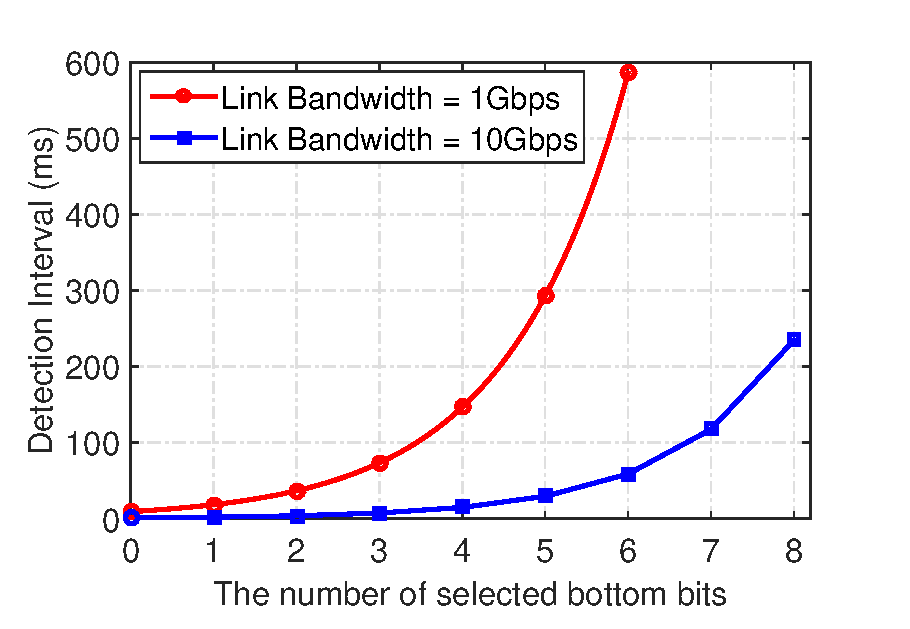
\includegraphics[width=0.65\columnwidth]{code_matlab/tmi2.eps}\\
  \caption{Detection interval $\emph{T}_{\emph{MI}}$ \emph{vs.} the number of selected bottom bits $\omega$.}\label{tmifig}
\end{figure}

\noindent{\textbf{End-host storage overhead.}}
For one session, {\tt S} stores the symmetric keys shared with entities on $\Psi$. With 128 bits length of each secret key, 16(n+1) bytes is occupied to store the keys. 
For each entity, two \emph{bloom filters} are established, resulting in extra storage overhead of 2(n+1)\emph{L} bytes in {\tt S}. So the source storage overhead for one session is (16+2\emph{L})(\emph{n}+1) bytes. On the destination host, only two \emph{bloom filters} should be stored for the packet sampling and localization, introducing its storage overhead of $\frac{2L}{8}$\emph{=}0.25\emph{L} bytes. 
Thus, {\tt S} and {\tt D} have storage overhead of O(n) and O(1) for the fixed bloom filter size \emph{L} per-session. With the average path length of the Internet, their storage overhead is 146.28 bytes and 3.28 bytes, respectively.
\vspace{-0.1in}
\subsection{Detection Interval}
\label{monitoringinterval}
When {\tt S} switches \emph{epoch} value, ReqProb packet is forwarded to all entities on $\Psi$ for requiring their packet sampling information. We respectively define $\emph{T}_{\emph{MI}}$ and $\emph{W}_\emph{B}$ as the detection interval and link bandwidth. As the existence of other sessions, there are at most $\frac{\emph{W}_\emph{B}}{\emph{P}_{\emph{size}}}$ packets of current session and $\frac{\emph{W}_\emph{B}}{2^\omega\cdot\emph{P}_{\emph{size}}}$ packets of each epoch, which can be delivered and sampled by entities per-second. Eq. \ref{tmi} shows the \emph{bloom filter} is consumed to the usage rate threshold $\xi_{\emph{th}}^\emph{e}$ after time interval $\emph{T}_{\emph{MI}}$. 
\begin{equation}\label{tmi}
\begin{split}
\frac{\emph{W}_\emph{B}}{2^\omega\cdot\emph{P}_{\emph{size}}}\cdot\emph{T}_{\emph{MI}} ~\emph{=~ L}\cdot\xi_{\emph{th}}^\emph{e}
~\Rightarrow~\emph{T}_{\emph{MI}} ~\emph{=}~\frac{{L}\cdot\xi_{\emph{th}}^\emph{e}\cdot2^\omega\cdot\emph{P}_{\emph{size}}}{\emph{W}_\emph{B}}
%&\Rightarrow\emph{T}_{\emph{MI}} ~\emph{=}~\frac{9.83\cdot10^6\cdot2^\mathcal{N}}{\emph{W}_\emph{B}}
\end{split}
\end{equation}
When \emph{L=}1 Kb, $\xi_{\emph{th}}^\emph{e}$\emph{=}80\%, \emph{P}$_{\emph{size}}$=1500 bytes and \emph{W}$_\emph{B}$ \emph{=}1 Gbps, we can learn $\emph{T}_{\emph{MI}}$ increases as $\mathcal{N}$ increases at the link bandwidth of both 1 Gbps and 10 Gbps, % ~\emph{=}~$9.375$\cdot2^\mathcal{N}$
as Fig. \ref{tmifig} shows. According to \cite{basescu2016high} \cite{tmi}, with the average value of 225 \emph{ms}, \emph{T}$_{\emph{MI}}$ between 100 \emph{ms} and 350 \emph{ms} conforms to the realistic network. In this case, $\omega$ \emph{=} 5, $\emph{T}_{\emph{MI}}$ \emph{=} 292.97 \emph{ms} when \emph{W}$_\emph{B}$ \emph{=}1 Gbps and $\omega$ \emph{=} 8, $\emph{T}_{\emph{MI}}$ \emph{=} 234.38 \emph{ms} when \emph{W}$_\emph{B}$ \emph{=}10 Gbps meet the requirements of detection interval in realistic network, respectively. 
%\vspace{-0.1in}
\section{Performance Evaluation}
\label{performanceevaluation}
In this section, we will evaluate \name{}'s performance, including the localization accuracy, the performance of key sharing, and the performance of packet forwarding with \name{}.\\
%, and localization accuracy when performing fault localization.}\\
\noindent {\bf Experiment setup.} We implement \name{} protocol described in Section \ref{lakeysection}, \ref{sourceandpathverificationsection} and \ref{faultlocalization} with \namekey{} as a user-level application for carrying out secret key distribution, source and path verification, and fault localization. The prototype of the router, called \name{} router, is implemented by using Click Modular Router \cite{kohler2000click}, which runs on Ubuntu Linux 12.04 with Intel(R) Core(TM) i5-4590, CPU @ 3.30 GHz, 16GB memory and NIC of 1000 Mbps\footnote{Of course, it is also feasible for the similar packet processing as \name{} to be implemented along fast TCAM path or in commercial router \cite{basescu2016high}.}. We achieve the communications between two computers acting as the source and the destination (Intel(R) Core(TM) i5-4200U, CPU @ 1.6GHz/2.3 GHz, 12.0 GB memory) through \name{} router. In this evaluation, we use SHA-3 algorithm to compute the hash values of long strings, such as the calculation of PacketID (see Eq. \ref{packetid}). For computing the PRF value, we use HMAC based on SHA-1. We respectively truncate the value of SHA-3 and HMAC to meet our requirements, such as from 256 bits to 128 bits for computing PacketID and from 160 bits to 32 bits for computing \emph{M}$_\emph{i}$. In \namekey{}, RSA algorithm is employed to compute the signature, asymmetric encryption, and decryption. To evaluate the effect of fault localization, such as localization accuracy, we implement a multi-hop simulation network using NS3, where the source communicates the detestation through more than one intermediate routing node.
\begin{figure*}[htbp]
\centering
\subfigure[The positive ratio of different router locations for different misbehaved packet loss probabilities.]{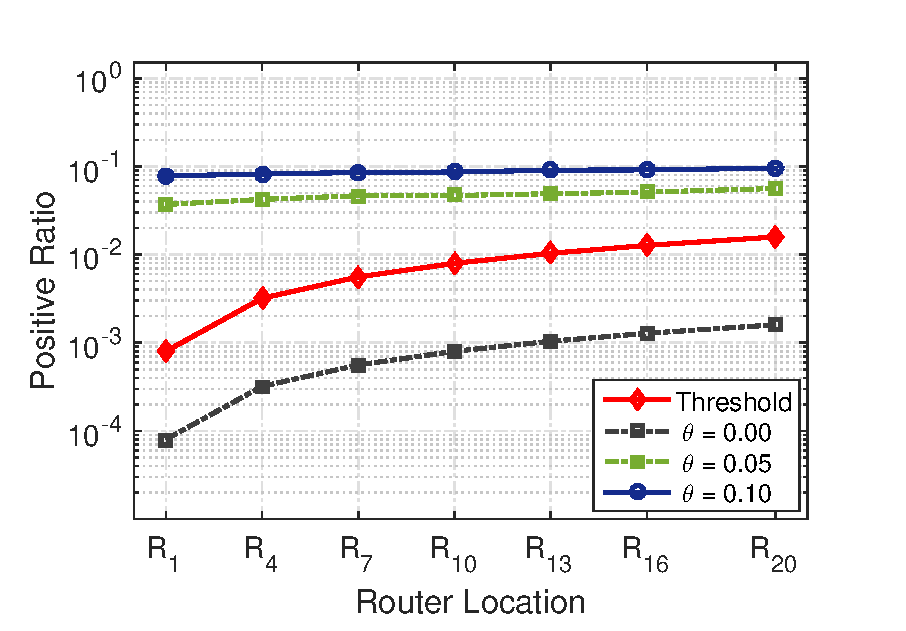
\includegraphics[width=2.3in, angle=0]{code_matlab/positiveratio11.eps}}\label{positiveratio}
\subfigure[The relationship between positive ratio and $~~~~$ $~~~~$ different packet natural loss probabilities.]{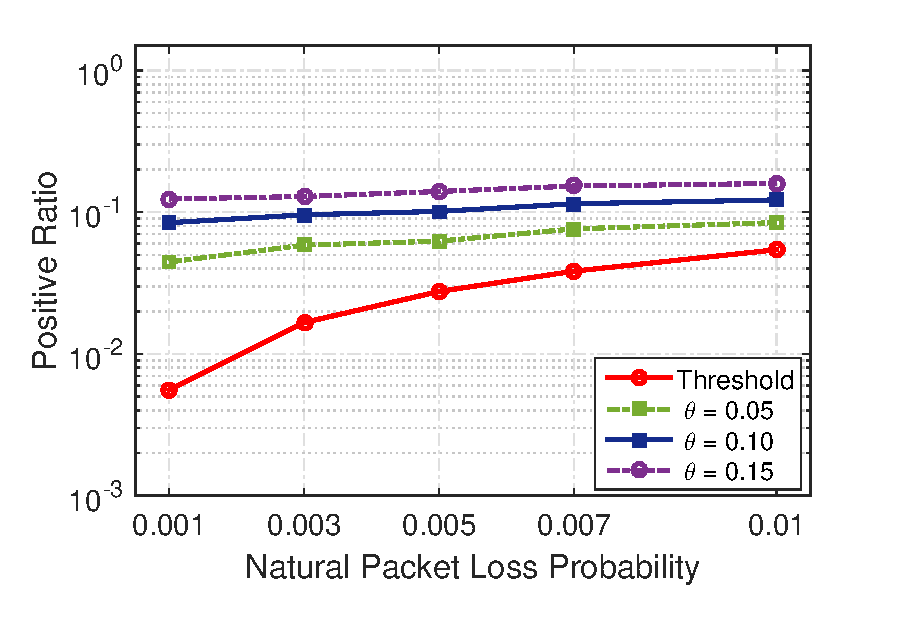
\includegraphics[width=2.3in, angle=0]{code_matlab/positiveratio22.eps}}\label{positiveratio2}
\subfigure[The localization accuracy for different packet $~~$ $~~~~$ mis-loss or natural loss probabilities.]{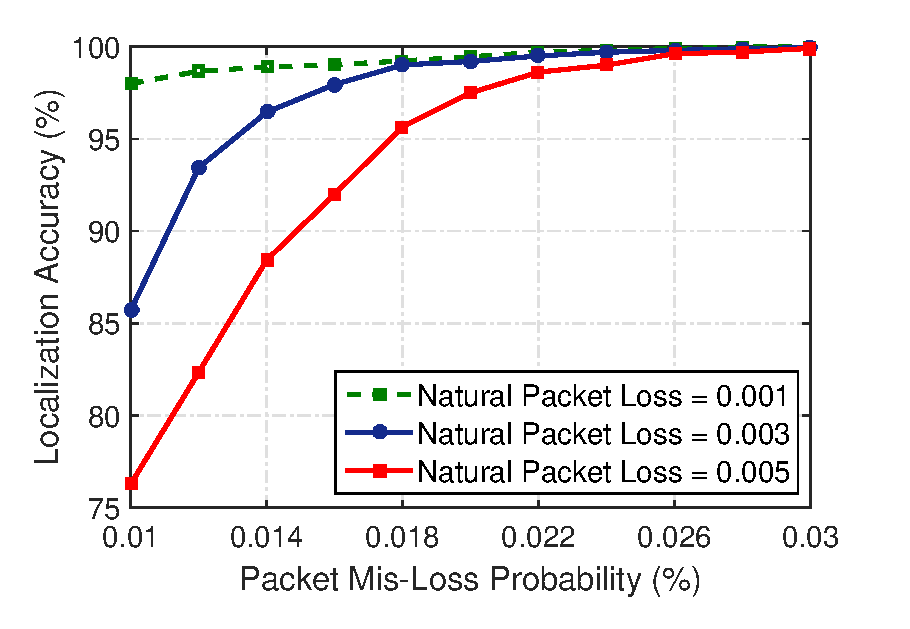
\includegraphics[width=2.3in, angle=0]{code_matlab/localizationaccuracy.eps}}\label{localizationaccuracyfig1}
\subfigure[The relationship between localization accuracy $~~~~$ and natural packet loss probability.]{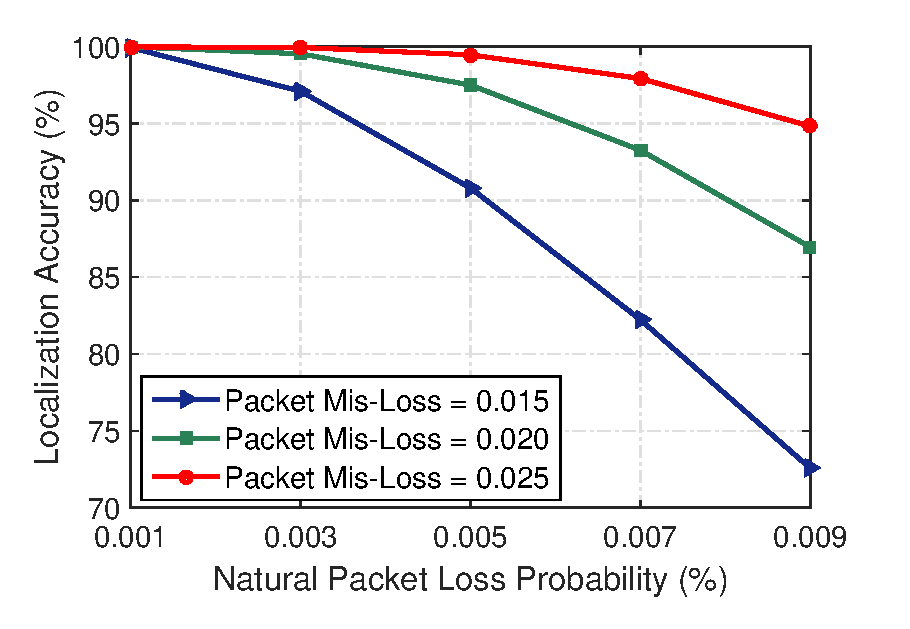
\includegraphics[width=2.3in, angle=0]{code_matlab/localizationaccuracy2.eps}}\label{localizationaccuracyfig2}
\subfigure[\name{} router's forwarding efficiency for different packet sizes under the Internet average path length.]{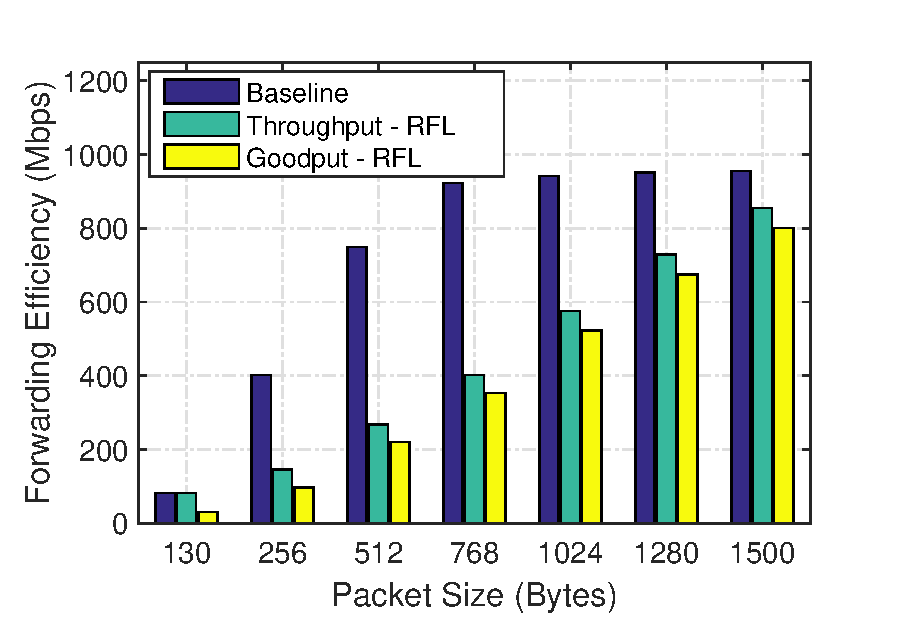
\includegraphics[width=2.3in, angle=0]{code_matlab/throughput2_spmoni.eps}}\label{packetsizeforwarding}
\subfigure[\name{} router's forwarding efficiency under different path lengths for the packet size of 1500 bytes.]{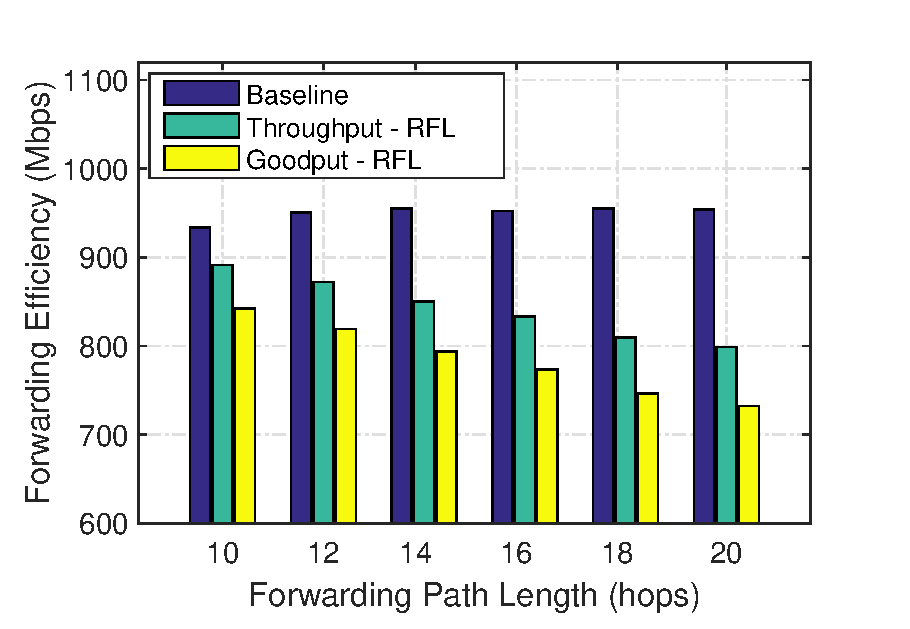
\includegraphics[width=2.3in, angle=0]{code_matlab/throughput_pathlength_spmoni2.eps}}\label{pathlengthforwarding}
\caption{The \name{} performance evaluation in terms of positive ratio, localization accuracy of fault localization, and \name{} router's forwarding efficiency.}\label{rflevaluation}
\end{figure*}
\vspace{-0.1in}
\subsection{Positive Ratio threshold}
\label{positiveratiothreshold}
%We define \emph{\textbf{positive ratio}} denoted by $\mathcal{P}_\emph{i}$ and $\mathcal{P}_\emph{D}$ for \emph{R}$_\emph{i}$ and {\tt D}, which illustrates the probability that the corresponding entity is misbehaved. When $\mathcal{P}_\emph{i}$ is larger than \emph{\textbf{positive ratio threshold}} (denoted by $\zeta$), and $\mathcal{P}_\emph{1}$, $\cdots$, $\mathcal{P}_{\emph{i-}1}$ are all less than $\zeta$, we can identify \emph{R}$_\tau$ or \emph{R}$_{\emph{i-}1}$ as the misbehaved entity (detailed in Section \ref{faultlocalization}).
We evaluate positive ratio threshold $\zeta_\emph{i}$ of $\emph{R}_\emph{i}$ through the simulation network with the path length of 20 hops, the longest forwarding path in end-to-end communication according to a CAIDA research \cite{huffaker2002distance}. The ratio illustrates the probability that the corresponding entity is misbehaved. When $\mathcal{P}_\emph{i}$ is larger than $\zeta_\emph{i}$, and $\mathcal{P}_\emph{1}$, $\cdots$, $\mathcal{P}_{\emph{i-}1}$ are respectively less than $\zeta_\emph{1}$, $\cdots$, $\zeta_{\emph{i-}1}$, we can identify \emph{R}$_\emph{i}$ or \emph{R}$_{\emph{i-}1}$ as the misbehaved entity (detailed in Section \ref{faultlocalization}). In \name{}, the attacks (including source spoofing, path hijacking, frame, and collusion attack) all lead to downstream entities' dropping the packet. %We respectively define $\theta$, $\theta_{\emph{na}}$ and $\theta_{\emph{mis}}$ as the probability of packet loss, natural loss and malicious loss (mis-loss) of the entity (including its upstream neighbored link).\\
\iffalse
\begin{figure}%[H]
  % Requires \usepackage{graphicx}
  \centering
  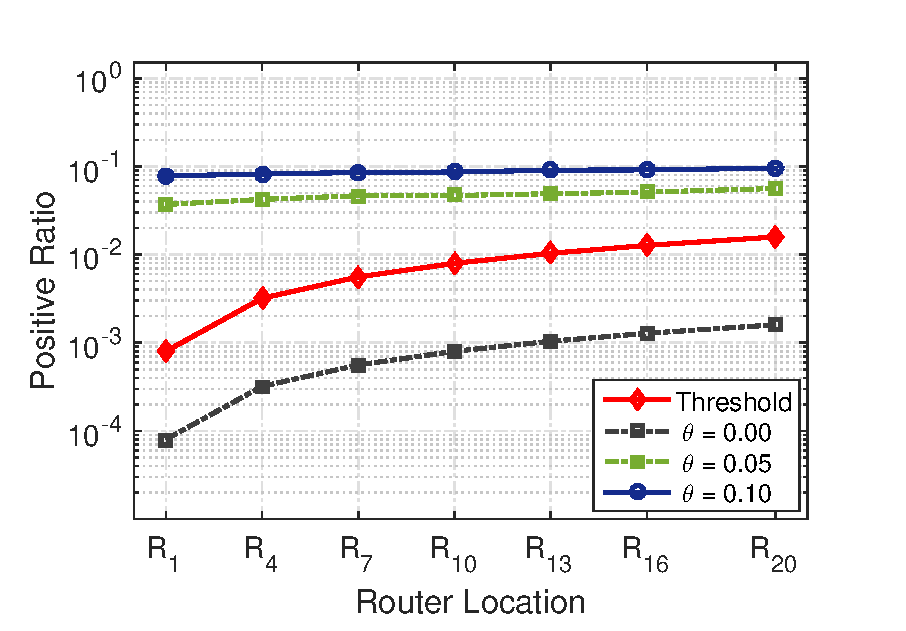
\includegraphics[width=0.85\columnwidth]{code_matlab/positiveratio11.eps}\\
  \caption{The relationship between router location (from \emph{R}$_1$ to \emph{R}$_\emph{20}$) and positive ratio with the variation of misbehaved packet loss probability.}\label{positiveratio}
\end{figure}
\begin{figure}%[H]
  % Requires \usepackage{graphicx}
  \centering
  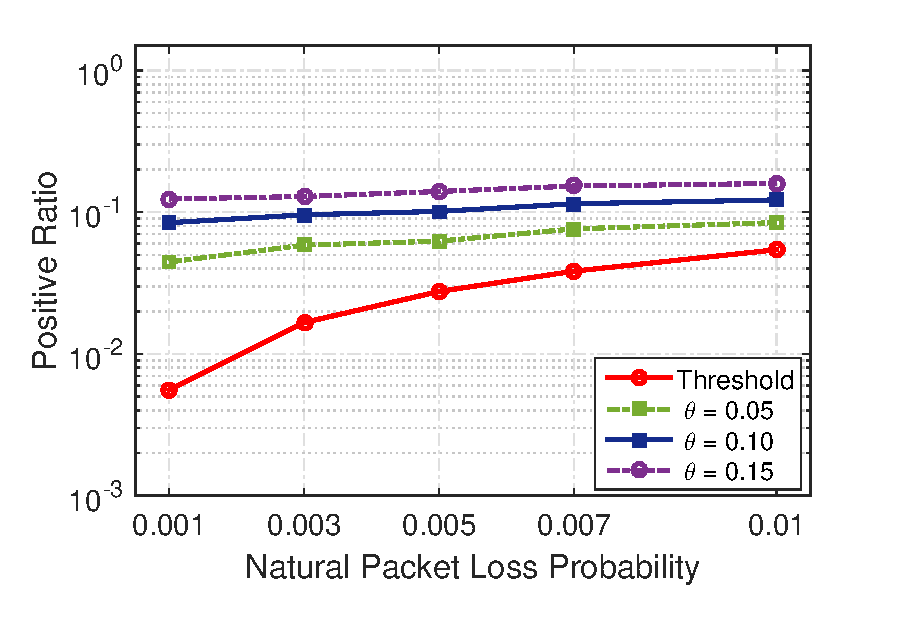
\includegraphics[width=0.85\columnwidth]{code_matlab/positiveratio22.eps}\\
  \caption{The relationship between natural packet loss probability and positive ratio with the variation of misbehaved packet loss probability.}\label{positiveratio2}
\end{figure}
\fi

Fig. \ref{rflevaluation}(a) shows the relationship between router location and its positive ratio with the variation of packet loss probability. To obtain a more accurate result, we run our simulation over 100 times for each result. The red line depicts the scenarios only with natural packet loss ($\theta_{\emph{na}}$=0.001), which is also the threshold line that helps identify the misbehaved entity. When the packet loss probability is 0.00, the positive ratio $\mathcal{P}$ is lower than the threshold value, because the lower packet loss probability brings about less packet loss during the transmission. We set one misbehaved router at different locations from \emph{R}$_1$ to \emph{R}$_{\emph{20}}$. The blue line ($\theta$=0.10) and the green dotted line ($\theta$=0.05) respectively show the positive ratio $\mathcal{P}$ of the misbehaved router in different locations. We learn that the positive $\mathcal{P_\emph{i}}$ will exceed the threshold $\zeta_\emph{i}$ when the malicious router behaves abnormally with the probability of $\theta$=0.10 or $\theta$=0.05. According to this threshold, {\tt S} can locate the misbehaved router who has different mis-loss probabilities.

We also evaluate the relationship between positive ratio and natural packet loss probabilities under different misbehaved packet loss probability. Fig. \ref{rflevaluation}(b) shows the positive ratio of the middle entity (i.e., \emph{R}$_\emph{7}$) with the average Internet forwarding path length, i.e., \emph{n}=13 hops. With the increment of natural packet loss probability, the positive ratio threshold becomes larger, because the higher loss probability introduces more packets to be dropped. When the misbehaved packet loss probability is larger than the natural loss probability, the corresponding ratios exceed the threshold value. Therefore, under different natural packet loss probabilities, the fault can also be localized in \name{} protocol.
\vspace{-0.1in}
\subsection{Fault Localization Accuracy}
\label{localizationaccuracy}
Based on the positive ratio threshold above, we evaluate the fault localization accuracy denoted by $\delta$ through a simulation scenario with 13-hop forwarding path. We set one router of random location on forwarding path as the misbehaved router, that can launch both source spoofing and path inconsistency attacks. Besides, this misbehaved router can also disturb \name{} protocol, which finally introduces the packets dropping.\\
\indent
We first evaluate the fault localization accuracy with the variation of packet mis-loss probability of misbehaved router, just as Fig. \ref{rflevaluation}(c) shows. From Fig. \ref{rflevaluation}(c), we can learn the fault localization accuracy of \name{} becomes higher with the increase of packet mis-loss probability. This is because more packet mis-loss results in higher positive ratio than the threshold, and the higher mis-loss probability make \name{} easier to identify the fault. We respectively take the value of natural packet loss probability as 0.001, 0.003 and 0.005, which introduce different positive ratio thresholds (described in Section \ref{positiveratiothreshold}). From Fig. \ref{rflevaluation}(c), we know less natural packet loss brings about higher localization accuracy, as the lower positive ratio threshold makes it easier to localize the fault. This is in line with our theoretical analysis in Section \ref{localizationaccuracyanalysis}.\\
\indent
Then the relationship between localization accuracy and natural packet loss probability is evaluated in Fig. \ref{rflevaluation}(d). With the larger range of natural packet loss, we can learn localization accuracy becomes lower when the more natural packet is dropped. Fortunately, under the smaller natural packet loss probability, such as 0.001 or 0.003, \name{} achieves the fault localization with the accuracy of over 99.5\% when the mis-loss probability is 0.020 or more.
\begin{table}
\caption{\namekey{} Evaluation - Communication Overhead}
\renewcommand\arraystretch{1.5}
\centerline{
\begin{tabular}{|p{1.8cm}<{\centering}|p{1.2cm}<{\centering}|p{1.2cm}<{\centering}|p{1.2cm}<{\centering}|}
%\toprule[2pt]
\hline
\hline
%\cline{1-1}
\centering
~&\textbf{\namekey{}} & \textbf{DRKey} & \textbf{ICING} \\\hline \hline
Source ({\tt S}) & 2 & 2 & 4$\ast$\emph{n}+4          \\\hline
Router (\emph{R}$_\emph{i}$) & 2 & 2 & 4$\ast$\emph{n}+4          \\\hline
Destination ({\tt D}) & 2 & 2 & 4$\ast$\emph{n}+4          \\\hline
%\bottomrule[2pt]
\hline
\end{tabular}
}
\begin{tablenotes}
  \item[1] Here, the communication overhead is evaluated by the number of extra packets during symmetric key distribution.
\end{tablenotes}
\label{communicationoverhead}
\end{table}
\vspace{-0.1in}
\subsection{Router Throughput and Goodput}
\label{routerthroughput}
We implement the prototype of \name{} router to evaluate the forwarding efficiency, including throughput and goodput, which can be used to demonstrate the technical feasibility in real experiments.
In order to evaluate the packet forwarding efficiency at routing entities, we use iperf \cite{tirumala2005iperf} to achieve the communications between the source and the destination through \name{} router. \name{} router performs the following operations when delivering packets: source and path validation, probabilistic packet sampling and storing sampling information. \\
\indent
From Eq. \ref{mid}, we learn the computation overhead of \name{} router increases linearly from \emph{R}$_\emph{n}$ to \emph{R}$_\emph{1}$ when recomputing the markings. Namely, \name{} routers close to {\tt S} have higher computation overhead than the router close to {\tt D} as the longer input. In this case, we evaluate the performance of middle router \emph{R}$_{[\frac{\emph{n}}{2}]}$ for the average-case analysis with different path lengths and packet sizes. Fig. \ref{rflevaluation}(e) shows the relationship between packet size and forwarding efficiency with the average Internet path length of 13 hops. We calculate goodput as the valid throughput of useful packet data, excluding \name{} header. Note that the smallest packet size is 130 bytes, including 90-byte \name{} header and 40-byte IP/TCP header. We adjust packet size of 130 bytes to 1500 bytes by configuring the interface Maximum Transmission Unit (MTU) sizes. From Fig. \ref{rflevaluation}(e), we can know both throughput and goodput of \name{} router increase with the improvement of packet size. Especially for the large packet of 1500 bytes, \name{} router can achieve over 90\% throughput and about 85\% goodput of baseline. From \cite{huffaker2002distance}, we learn that the path length of end-to-end communication is 15.3 $\pm$ 4.2 hops for IPv4 packets. Thus, we evaluate the packet forwarding efficiency with the path length of 10 hops to 20 hops in Fig. \ref{rflevaluation}(f). We can learn that \name{} router's throughput and goodput all decrease when the forwarding path length increases because more downstream routers' markings are added as the input of marking recomputation. The longer input of marking recomputation incurs lower forwarding efficiency. Concretely, with path length increment of 1 hop, the throughput and goodput will reduce by 9.26 Mbps. Fortunately, the throughput and goodput respectively exceed 850 Mbps and 800 Mbps in the networks of 13-hop path length, more than 90\% and 85\% compared to the baseline. Thus \name{} incurs only 10\% forwarding efficiency while guaranteeing the robustness of fault localization, which is an incomparable advantage of other packet verification mechanism.
\begin{table}
\caption{\namekey{} Evaluation - ReqKey and AckKey Packet Latency}
\renewcommand\arraystretch{1.5}%{\multirowsetup}{\centering}
\centerline{
\begin{tabular}{|p{1.6cm}<{\centering}|p{1.8cm}<{\centering}|p{1.7cm}<{\centering}|p{1.7cm}<{\centering}|} %|r|c|l|}%\multirow{5}{2cm}{Source}
%\toprule[2pt]
\hline
\hline
%\cline{1-1}
\centering
&\textbf{Entity} & \textbf{Path Length} & \textbf{Latency} \\\hline \hline
& Source ({\tt S})  & Irrelevant           & 653 $\mu$s           \\\cline{2-4}
ReqKey & Router (\emph{R}$_\emph{i}$) & Irrelevant          & 548 $\mu$s           \\\cline{2-4}
& Destination ({\tt D})  & Irrelevant          & 627 $\mu$s           \\\hline \hline
& & 11           &  13128 $\mu$s           \\\cline{3-4}
& & 13           &  16534 $\mu$s           \\\cline{3-4}
& Source ({\tt S}) & 15           &  20176 $\mu$s           \\\cline{3-4}
AckKey &                 & 17           &  24051 $\mu$s           \\\cline{3-4}
&                 & 19           &  28815 $\mu$s           \\\cline{2-4}
& Router (\emph{R}$_\emph{i}$)  & Irrelevant          & 903 $\mu$s           \\\cline{2-4}
& Destination ({\tt D})         & Irrelevant          & 754 $\mu$s           \\\cline{2-4} \hline\hline
%\bottomrule[2pt]
\end{tabular}
}
\label{ackkeypacketlatencytable}
\end{table}
\vspace{-0.1in}
\subsection{Performance and Overhead of \namekey{}}
\label{laskeyevaluation}
To demonstrate the feasibility of \namekey{} in the early stage of \name{} protocol, we perform \namekey{} performance evaluation during symmetric key distribution. The evaluation results show that \namekey{} introduces the low communication overhead and packet latency. %The storage overhead has been analyzed in Section \ref{storageoverhead}.

Table \ref{communicationoverhead} provides the results of communication overhead (evaluated by the number of extra packets) at the source ({\tt S}), the router (\emph{R}$_\emph{i}$) and the destination ({\tt D}). We can learn \namekey{} achieves the same lower communication overhead with the state-of-the-art scheme DRKey \cite{kim2014lightweight}, and outperforms than ICING \cite{naous2011verifying}. Note that \namekey{} and DRKey all require only 2 additional packets as the communication overhead for the symmetric key establishment, while ICING needs 4$\ast$\emph{n}+4 extra packets on all entities.

More importantly, \namekey{} achieves a more secure and robust symmetric key distribution than the state-of-the-art scheme DRKey. On one hand, if any misbehaved router disturbs secret key distribution by means of dropping, modifying or redirecting \emph{request} or \emph{ack} packet, DRKey scheme will fail. However, \namekey{} enables each entity to verify the \emph{request} or \emph{ack} message. If any failure occurs or the timer expires, the entity will send its encrypted symmetric key back to {\tt S}. In this case, {\tt S} can still obtain reliable entities' symmetric key even if there is any router trying to disturb secret key establishment. On the other hand, if any misbehaved router disturbs key distribution, DRKey will be stranded, resulting in {\tt S}'s wasting time to wait for ack message. However, \namekey{} can realize it as soon as possible with the help of timer, and localize the fault who disturbs secret key distribution. In this case, {\tt S} can adjust the policies (e.g., avoiding the localized misbehaved router or correcting the fault) based on the result of fault localization.
\iffalse
\begin{table}
\caption{\namekey{} Evaluation - ReqKey Packet Latency}
\renewcommand\arraystretch{1.5}
\centerline{
\begin{tabular}{|p{2cm}<{\centering}|p{2cm}<{\centering}|p{2cm}<{\centering}|p{2cm}<{\centering}|}
%\toprule[2pt]
\hline
\hline
%\cline{1-1}
\centering
\textbf{Entity} & \textbf{Path Length} & \textbf{Latency} \\\hline \hline
Source ({\tt S})  & Irrelevant           & 653 $\mu$s           \\\hline
Router (\emph{R}$_\emph{i}$) & Irrelevant          & 548 $\mu$s           \\\hline
Destination ({\tt D})  & Irrelevant          & 627 $\mu$s           \\\hline
%\bottomrule[2pt]
\hline
\end{tabular}
}
\label{reqkeypacketlatency}
\end{table}
\fi

To evaluate packet latency during \namekey{} processing, we implement the prototype of \namekey{} on the source host, the RFL router, and the destination host. \namekey{} scheme contains two stages: ReqKey stage and AckKey stage. From Section \ref{reqkeytransmission}, we can learn the packet latency on different entities is irrelevant to path length on ReqKey stage. In this case, we will ignore the effect of path length changes on entities' performance. \\
\indent Table \ref{ackkeypacketlatencytable} shows the packet latency of ReqKey stage and AckKey stage on the source, intermediate routers, and the destination. We can learn the packet latency of \namekey{} on the source is affected by path length, especially on AckKey stage. That is mainly because the source will check all the signatures and decrypts the encrypted symmetric keys when receiving AckKey packet, leading to higher computation overhead in proportion to path length. This result also shows the packet latency on RFL router is smaller than at least one of end hosts, which enables more cycles to be used to distribute secret keys by the source or the destination. 
\iffalse
\begin{figure}%[H]
  % Requires \usepackage{graphicx}
  \centering
  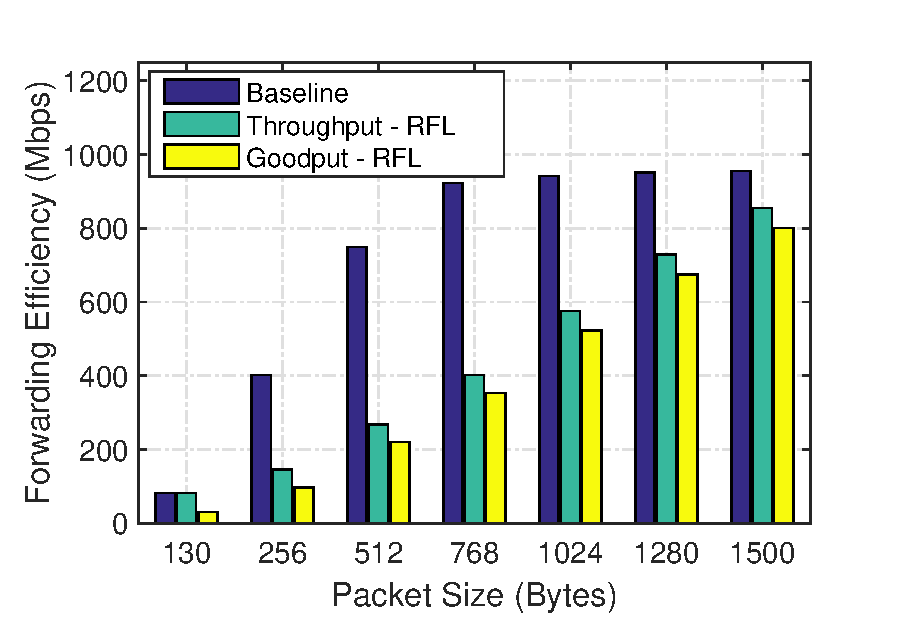
\includegraphics[width=6cm]{code_matlab/throughput2_spmoni.eps}\\
  \caption{\name{} router's forwarding efficiency (throughput and goodput) for IPv4 packets of 130 bytes to 1500 bytes, with the path length of 13 hops.}\label{packetsize}
\end{figure}
\begin{figure}%[H]
  % Requires \usepackage{graphicx}
  \centering
  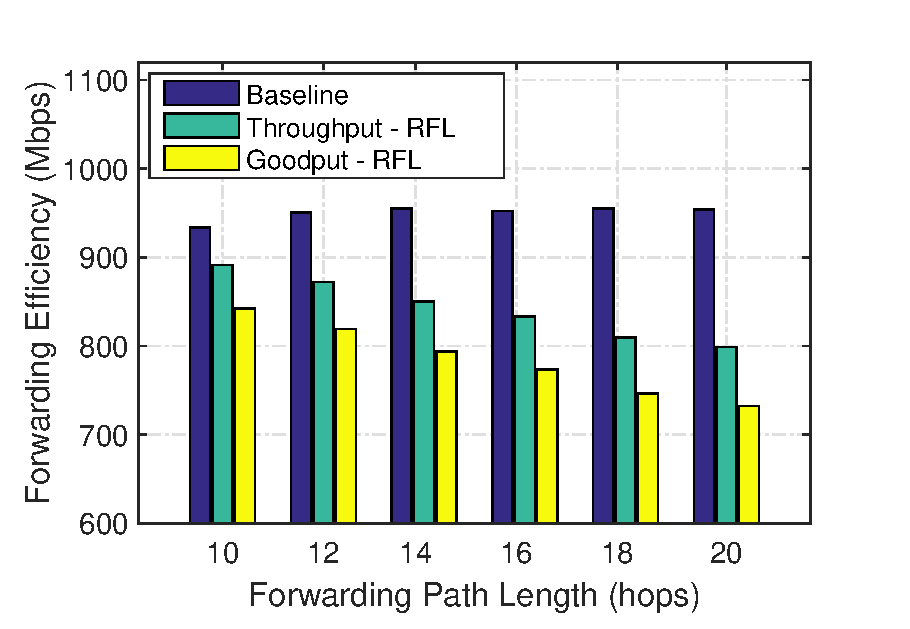
\includegraphics[width=6cm]{code_matlab/throughput_pathlength_spmoni2.eps}\\
  \caption{\name{} router's forwarding efficiency (throughput and goodput) for data-plane networks of 10 hops to 20 hops, with packet size of 1500 bytes.}\label{pathlength}
\end{figure}
\begin{figure}%[H]
  % Requires \usepackage{graphicx}
  \centering
  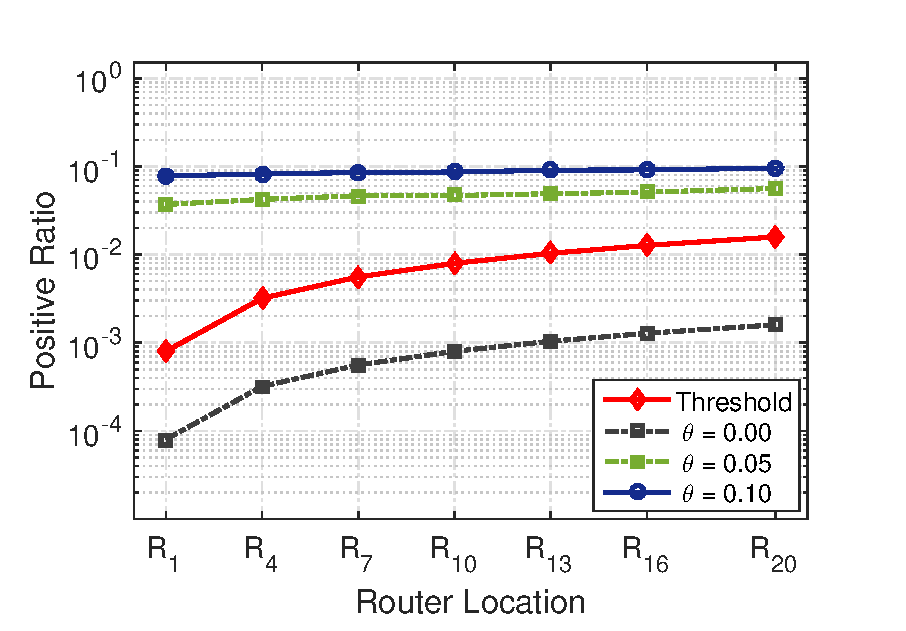
\includegraphics[width=6cm]{code_matlab/positiveratio11.eps}\\
  \caption{The relationship between router location (from \emph{R}$_1$ to \emph{R}$_\emph{20}$) and positive ratio with the variation of misbehaved packet loss probability.}\label{positiveratio}
\end{figure}
\begin{figure}%[H]
  % Requires \usepackage{graphicx}
  \centering
  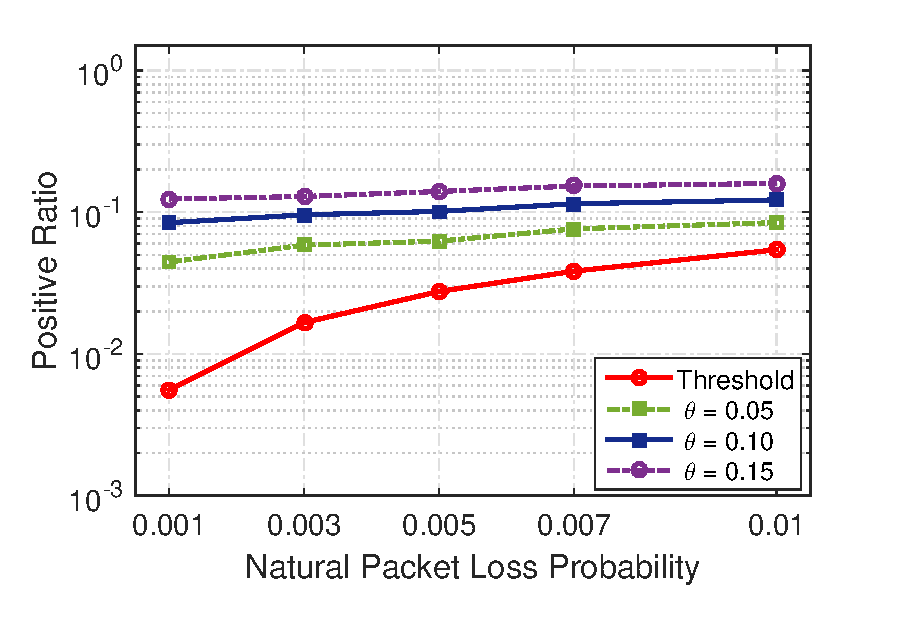
\includegraphics[width=6cm]{code_matlab/positiveratio22.eps}\\
  \caption{The relationship between natural packet loss probability and positive ratio with the variation of misbehaved packet loss probability.}\label{positiveratio2}
\end{figure}
\begin{figure}%[H]
  % Requires \usepackage{graphicx}
  \centering
  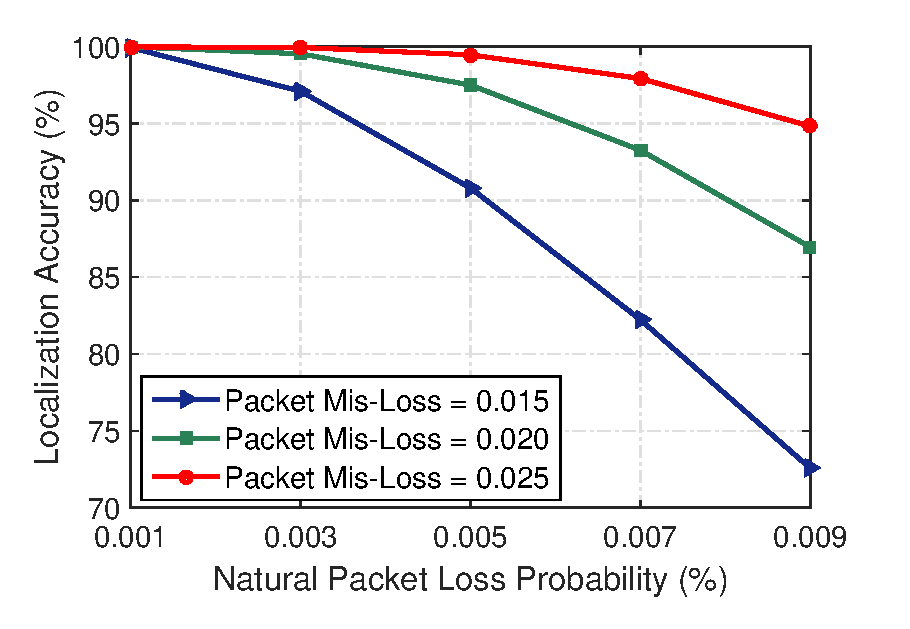
\includegraphics[width=6cm]{code_matlab/localizationaccuracy2.eps}\\
  \caption{The relationship between localization accuracy $\delta$ and natural packet loss probability with the different packet mis-loss simulation scenario.}\label{localizationaccuracyfig2}
\end{figure}
\begin{figure}%[H]
  % Requires \usepackage{graphicx}
  \centering
  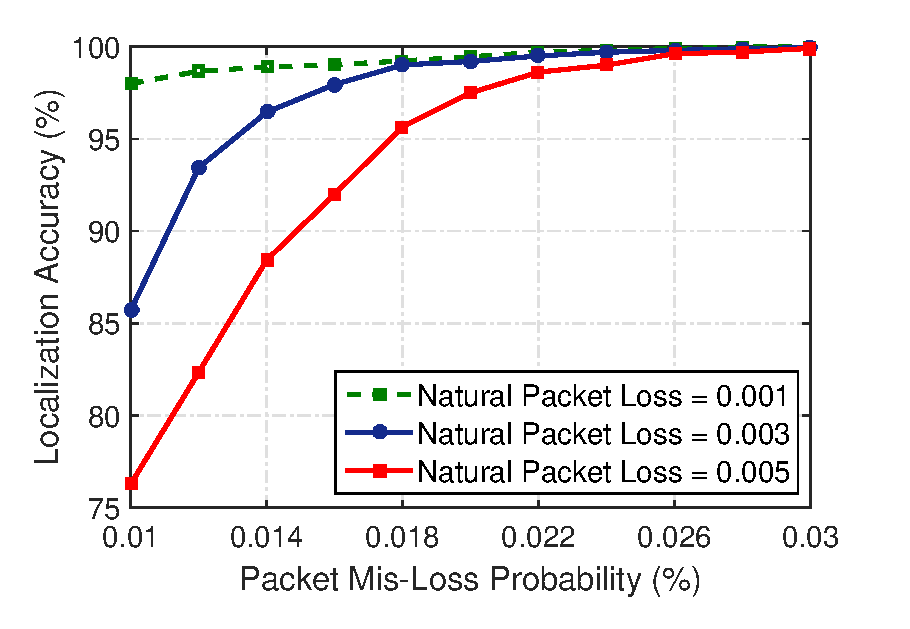
\includegraphics[width=6cm]{code_matlab/localizationaccuracy.eps}\\
  \caption{The relationship between localization accuracy $\delta$ and packet mis-loss probability with different natural packet loss in simulation scenario.}\label{localizationaccuracyfig1}
\end{figure}
\fi
%\vspace{-0.1in}

%\vspace{-0.1in}
\section{Discussion}
\label{discussion}
\noindent\textbf{Asymmetric paths.} We mainly describe the fault localization for the packet verification with symmetrical paths, while many forwarding paths between the source and the destination in the current Internet are asymmetric \cite{john2010estimating} \cite{de2015asymmetric} \cite{wassermann2016analysis}. \name{} can also provide the compatibility for asymmetric paths. With the asymmetric paths, the timer $\mathcal{T}_\emph{i}$ will expire as \emph{R}$_\emph{i}$ does not receive AckKey or AckProb packets from its downstream entities. In this case, \emph{R}$_\emph{i}$ then creates and initializes \emph{AckKey}$_\emph{i}$ or \emph{AckProb}$_\emph{i}$, which will be delivered to the source. Based on the encrypted symmetric keys or sampling information, the source can also identify and localize the misbehaved entity (see Algorithm \ref{positiveratebasedfaultlocalization}).

\noindent\textbf{Forwarding path instability.} \name{} enable the source to pre-insert the markings of entities on $\Psi$ into \name{} header for later packet verification. There is still a probability that the forwarding path $\Psi$ changes due to the link failure, network congestion, and misconfiguration, making both the packets dropped incorrectly and the fault localized wrongly. Fortunately, the network end-to-end communications keep stable from tens of minutes to several days \cite{cunha2011measuring} \cite{kang2013crossfire}. Besides, the stable forwarding paths (longer than 6 hours) will be chosen to transmit packets for 96\% of times \cite{cunha2011measuring}. To further address this problem, the source and perform \namekey{} several times until it can obtain symmetric keys of all entities on the latest purposed path $\Psi$. Using the newly obtained symmetric keys, \name{} provides a better compatibility for network instability.

\noindent\textbf{Tradeoff between robustness and overhead.} In \name{}, there is a conflict between robustness and overhead. On one hand, to ensure the robustness against unreliable communication channels, \name{} introduces the timer for each entity, which also incurs an extra overhead. Fortunately, \name{} enables each entity to use its timer only receiving request packets (i.e., ReqKey and ReqProb). This can help to lower the overhead of each entity to a certain extent. On the other hand, each entity has to store bloom filters for sampling packets. However, we think the packet sampling operation is an essential element for constructing robust fault localization. Through our analysis in Section \ref{storageoverhead}, the average storage overhead of each entity is within an acceptable range, fortunately.

\noindent\textbf{Incremental deployment.} As the packet verification is performed hop by hop, \name{}'s incremental deployment makes source and path verification paralyzed. However, it does not affect packets sampling when the entities that do not deploy \name{} ignore the packet verification. In this case, the source can still obtain the sampling information of entities and localize the fault. Due to lacking a part of sampling information, the source can only narrow the scope of the fault, which also contributes to constructing a reliable packet delivery.
\section{Related Work}
\label{relatedwork}
\noindent{\textbf{Secure routing and forwarding.}}
Routing security has been widely studied to ensure correct packet forwarding on the Internet~\cite{kent2000secure} \cite{hu2004spv} \cite{goodell2003working} \cite{ng2004extensions} \cite{candolin2005packet} \cite{hu2013general}. S-BGP \cite{kent2000secure} verified the authenticity of announced routing paths by signing them, which incurs significant computation and communication overhead. In order to reduce the costs, a large amount of variants have been proposed. For example, So-BGP \cite{ng2004extensions} ensured correctness of announced routing paths by leveraging network topologies. IRV~\cite{goodell2003working} validated the correctness of the announced routing paths by establishing an additional IRV server in each AS, which limited its deploymentability. All these approaches did not address the security of routing data plane.\\
%which brings about the difficulties and challenges of maintenance and migration.
\noindent{\textbf{Source and path verification.}}
%There are many researches about source authentication and path validation.
%A scalable and secure OPT (
Origin and Path Trace (OPT) protocol \cite{kim2014lightweight} \cite{zhang2014mechanized} allows each router to verify delivered packets so as to verify correctness of packet source and forwarding paths. It reduced storage overhead in routers, which prevents state exhaustion attack. Naous et. al., \cite{naous2011verifying} proposed a Path Verification Mechanism (PVM) %to achieve the source and path verification,
to validate whether the packets correctly forwarded their forwarding paths. Cai et. al.,~\cite{cai2015source} performed source authentication and path validation by leveraging a set of orthogonal sequences instead of lightweight cryptographic operations. Unfortunately, these mechanism cannot localize the detected faults.
%Moreover, they might be v if they run in unreliable networks ({\bf LQ: double check, and tell more specific points.}) and . %the fault localization service, ignoring the investigation of the error. Other methods, such as
Although Passport \cite{liu2008passport} and SNAPP \cite{barak2008protocols} did not have such a  problem, they were vulnerable to source spoofing or path deviation attacks.\\
%cannot provide both packet source and forwarding path  or verify one aspect of source authenticity and path consistency.
\noindent{\textbf{Fault localization.}}
%To locate the misbehaved router or link, Adrian Perrig \emph{et al.} have carried out much research to
There are a large amount of studies on locating data plane errors~\cite{basescu2016high}~\cite{zhang2012shortmac}~\cite{zhang2012secure}~\cite{zhang2011network} \cite{wang2017smartfix}. Faultprints \cite{basescu2016high} was the first secure inter-domain fault localization scheme. It could localize the misbehaved links that drop, delay, modify packets at a high speed. ShortMAC \cite{zhang2012shortmac} leveraged probabilistic packet authentication to locate the illegal network links, which achieved low detection delay and incurred small overhead. DynaFL \cite{zhang2012secure} proposed the secure neighborhood-based fault localization (FL) protocol to  cope with dynamic traffic patterns and routing path with small router state. TrueNet \cite{zhang2011network} leveraged trusted computing technology to build a trusted network-layer architecture, and implemented a small TCB to address secure FL with small router state. However, these schemes might failed to localize faults if the generated acknowledgement packets are maliciously dropped by colluding entities. Our proposed protocol well addresses this issue by setting the timer on each entity, where the entity would send its sampling information towards {\tt S} once the timer expires. 
%\vspace{-0.1in}
\section{Conclusion}
\label{conclusionsection}
In this paper, we %\textcolor{red}%{propose fault localization for secure packet delivery even over unreliable communication channels, and} 
propose a robust data-plane fault localization protocol called \name{}, which achieves high accuracy for localizing the misbehaved entity even over unreliable communication channels. %\textcolor{red}{For building a reliable detection channel, 
\name{} leverages a robust symmetric key sharing scheme to ensure that all entities forwarding the same packets can synchronize their verification keys. 
%obtain on forwarding path.} %\textcolor{red}{\namekey{} contributes to building a reliable detection channels.} 
%Based on the symmetric keys, \name{} %includes a secure key distribution mechanism that can resist to interference from adversaries. By leveraging the keys, it
\name{} samples packets and embeds cryptographic markings in the packets so as to verify packet source and forwarding paths, and achieve fault localization, which ensures accuracy and robustness of the protocol even in the presence of interference from adversaries. We prototype \name{} and use real experiments based on the prototype to demonstrate the performance of \name{}. The results show \name{} achieves around 99.5\% localization accuracy, and incurs small communication overhead, e.g., more than 90\% throughput and 85\% goodput compared to the baseline. %Besides, \name{} also makes both packet and routing entity lightweight with 6.03\% packet overhead and 3.23 MB router storage overhead.
We hope that the robustness properties of \name{} can become a fundamental primitive to construct highly secure and efficient data-plane protocols. 
%\vspace{-0.1in}
\bibliographystyle{unsrt}
\bibliography{reference}

\end{document}